%%%%%%%%%%%%%%%%%%%%%%% file template.tex %%%%%%%%%%%%%%%%%%%%%%%%%
%
% This is a template file for Web of Conferences Journal
%
% Copy it to a new file with a new name and use it as the basis
% for your article
%
%%%%%%%%%%%%%%%%%%%%%%%%%% EDP Science %%%%%%%%%%%%%%%%%%%%%%%%%%%%
%
%%%\documentclass[option]{webofc}
%%% "twocolumn" for typesetting an article in two columns format (default one column)
%

\newcommand{\sqrts}{\ensuremath{\sqrt{s}}\xspace}
\newcommand{\sqrtsNN}{\ensuremath{\sqrt{\smash[b]{s_{_{\text{NN}}}}}}\xspace}
\newcommand{\PbPb}{\ensuremath{\mathrm{PbPb}}\xspace}
\newcommand{\pp}{\ensuremath{\Pp\Pp}\xspace}
\newcommand{\GeVc}{\ensuremath{\rm GeV/c}\xspace}
\newcommand{\raa}{\ensuremath{R_{\mathrm{AA}}}\xspace}
\newcommand{\rpa}{\ensuremath{R_{p \mathrm{A}}}\xspace}
\newcommand{\taa}{\ensuremath{T_{\mathrm{AA}}}\xspace}
\newcommand{\absy}{\ensuremath{ \abs{y}}\xspace}
\newcommand{\abseta}{\ensuremath{ \abs{\eta}}\xspace}
\newcommand{\Dzero}{\rm D^{0}\xspace}
\newcommand{\Bplus}{\rm B^{+}\xspace}
\newcommand{\Dzerodecay}{\rm D^{0} \rightarrow K^{-} \pi^{+}\xspace}
\newcommand{\Bplusdecay}{\rm \Bplus \rightarrow J/\Psi \hspace{0.1cm} K^{+} \rightarrow \mu^{+} \mu^{-} K^{+}}
\newcommand{\bdecayX}{\rm B \rightarrow J/\Psi \hspace{0.1cm}+ X}
\newcommand{\Ds}{\rm D_{s}^{+}\xspace}
\newcommand{\Lambdac}{\rm \Lambda_{c}\xspace}
\newcommand{\pt}{\rm p_{\rm T} \xspace}

\documentclass{webofc}
\usepackage[varg]{txfonts}   % Web of Conferences font
%
% Put here some packages required or/and some personnal commands
%
%
\begin{document}
%
\title{Heavy flavour production at RHIC and LHC}
%
% subtitle is optionnal
%
%%%\subtitle{Do you have a subtitle?\\ If so, write it here}

\author{\firstname{Gian Michele} \lastname{Innocenti}\inst{1}\fnsep\thanks{\email{ginnocen@cern.ch}} 
}

\institute{Massachusetts Institute of Technology}

\abstract{
In this proceedings, I present selected experimental results on heavy-flavour production at RHIC and at the LHC, which were 
presented at the Strangeness in Quark Matter 2017 conference. I will present a brief introduction to the heavy-flavour physics in 
heavy ion collisions and I will focus on recents measurements of in-medium energy loss and and collective properties of heavy-flavour  
particles, which provided important information on the mechanisms of heavy flavour interaction with the hot and dense medium 
created in ultra-relativistic heavy-ion collisions.
}
%
\maketitle
%
\section{Introduction}
\label{intro}
Heavy quarks are effective probes to study the properties of the deconfined medium created in heavy ion collisions\footnote{More details and a complete bibliography for this section can 
be found in~\cite{saporegravis}}. These quarks, as a consequence of their large masses, are mostly produced in primary hard QCD scatterings with a production 
timescale that is shorter than the formation time of the QGP. During their propagation through the medium, heavy quarks lose energy via radiative and collisional 
interactions with the medium constituents. QCD predicts that quarks lose less energy than gluons as a consequence of their smaller colour factor. 
In addition, the so-called ``dead-cone effect" is expected to reduce small-angle gluon radiation of heavy quarks when compared to both 
gluons and light quarks. Precise measurements of the nuclear modification factor \raa of particles containing both light and heavy quarks can thus 
provide important tests for the predicted flavour-dependence of in-medium energy loss. In addition, the measurement of the \raa of strange D mesons 
can also help estimating the relevance of the coalescence mechanism in which charmed hadrons are formed 
by the combination of charm quarks with light quarks from the medium. If coalescence plays a relevant role in the charm hadronisation, 
the yield of $\Ds$ particles are expected to be significantly enhanced with respect to the one of $\Dzero$ mesons at low-intermediate transverse momenta ($\pt$), 
as a consequence of the increased abundance of strange quarks in the deconfined medium. The production ratio of $\Lambdac/\Dzero$ 
is also expected to be enhanced with respect to that of charmed mesons under the assumption that di-quarks bounded states in the 
quark-gluon plasma can be formed. Finally, the study of the collective properties of D and B mesons through detailed measurements of their azimuthal coefficienct $v_{n}$ 
at low-intermediate $\pt$ can also help quantifying the extent to which charm and beauty quarks flow with the medium, 
which is a good measure of their interaction strength and  of their level of thermalisation.
\\ \\
The production of open heavy-flavours is measured at RHIC and at the LHC using several experimental techniques. Charm and beauty hadrons can me measured via the exclusive reconstruction 
of their hadronic or semi-leptonic decay channels (e.g. $\Dzerodecay$ or $\Bplusdecay$) or via the inclusive reconstruction of semi-leptonic decays (e.g. $\bdecayX$). The production of 
heavy-flavour particles can also be studied up to very high $\pt$ by measuring jets of hadrons produced in the fragmentation of a charm or beauty quark.  Charm and beauty decays are 
characterised by relativetely small cross sections and by decay vertices which are displaced few hundreds $\mu$m from the main interaction vertices.
Therefore the study of these observables requires very large statistics of minimum-bias and triggered events 
and precise tracking and vertexing detectors that can operate under conditions of very large detector occupancy. 
\section{Proton-proton measurements}
\label{ppmeasurements}
The study of heavy-flavour production in proton-proton collisions is considered a fundamental reference for nucleus-nucleus measurements but at the same time it provides
an important benchmark for perturbative QCD calculations based on a factorisation approach. The possibility of measuring the charm and beauty production both at RHIC and the LHC is crucial to constrain the relative relevance 
of different production mechanisms (e.g. flavour creation vs gluon fusion processes), which are expected to play a different role at different energies. The $\pt$- and $y$-differential cross sections of charm and beauty quarks were 
measured by several collaborations both at RHIC and at the LHC and were found to be consistent with perturbative QCD calculations (e.g. FONLL) that include a consistent description of next-to-leading order processes. 
As an example, in the left panel of Fig.~\ref{fig:ppresults}, the $\Dzero$ production cross sections as a function of $\pt$ measured by the ALICE experiment at LHC at 7 TeV and by the STAR experiment at RHIC at 200 and 500 GeV are presented. 
In the central panel of the same figure, the $\Bplus$ production measured by the ATLAS  experiment at 7 TeV is shown. Although theoretical calculations are able to describe successfully single-differential 
observables, more differential measurements like $\rm D \bar{D}$ or $\rm B \bar{B}$ azimuthal correlations showed that the current understanding of next-to-leading order processes at least at the LHC is still not satisfactory. In particular, 
the contribution of the gluon-splitting production mechanism ($g \rightarrow c\bar{c}$ or $g \rightarrow b\bar{b}$), which is dominant at small angles between the particle-anti-particle pairs is 
sizeably understimated by theoretical calculations (right panel of Fig.~\ref{fig:ppresults}). A better description of the gluon splitting processes would be extremely important since charm 
and beauty quarks produced via these mechanisms are mostly sensitive to the energy loss of gluons instead of that of the heavy parton. 
\begin{figure}[ht]
\centering
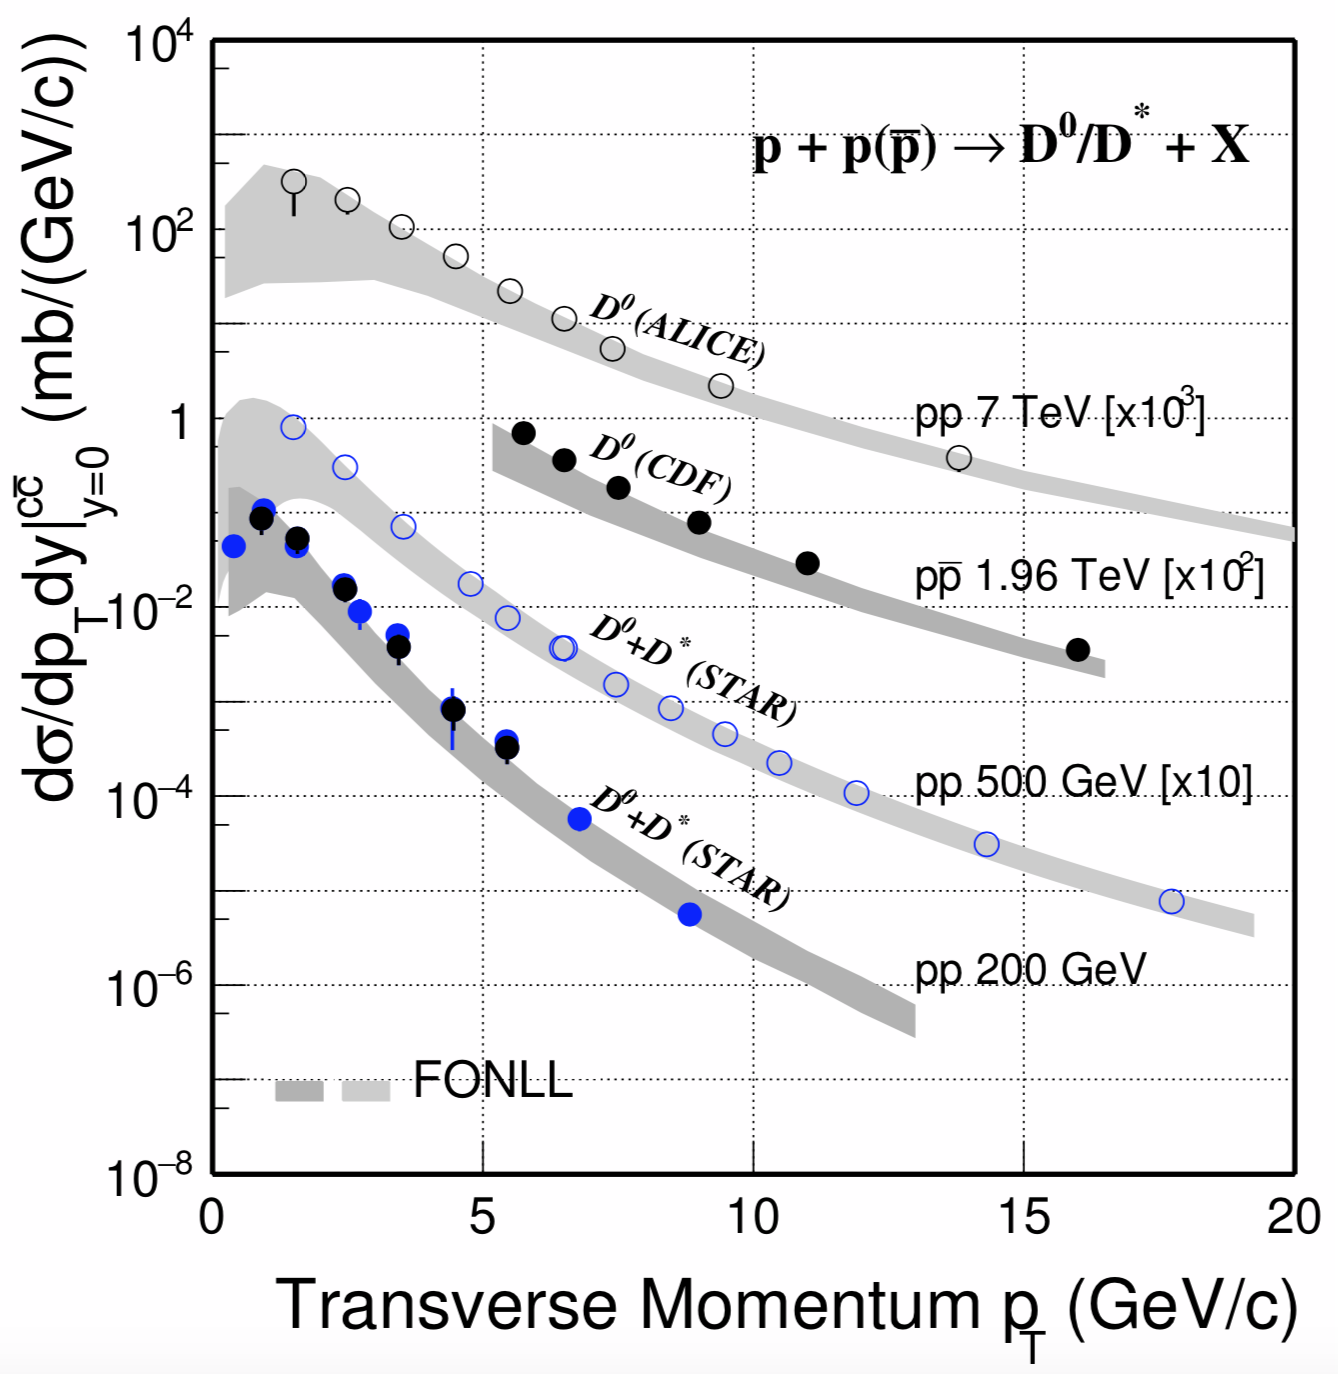
\includegraphics[width=.32\textwidth]{Plots/Dcross_sectionLHCRHIC}
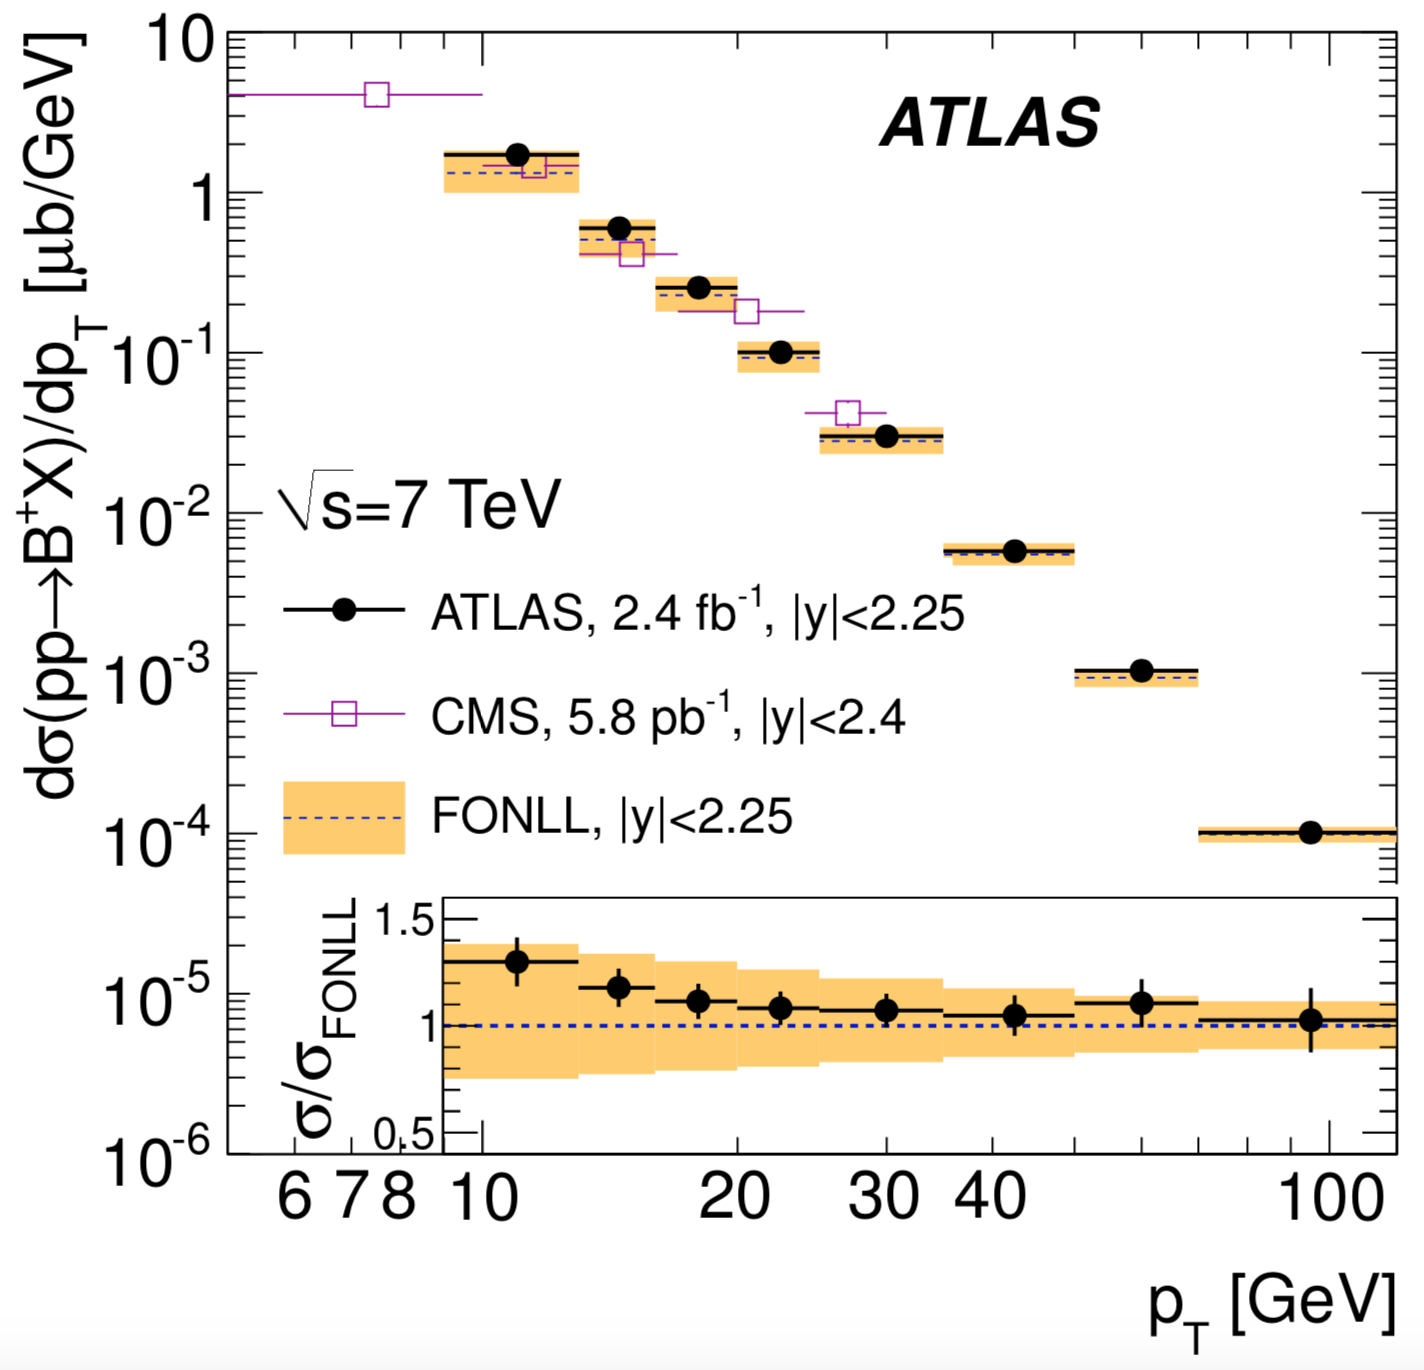
\includegraphics[width=.32\textwidth]{Plots/BplusATLASpp}
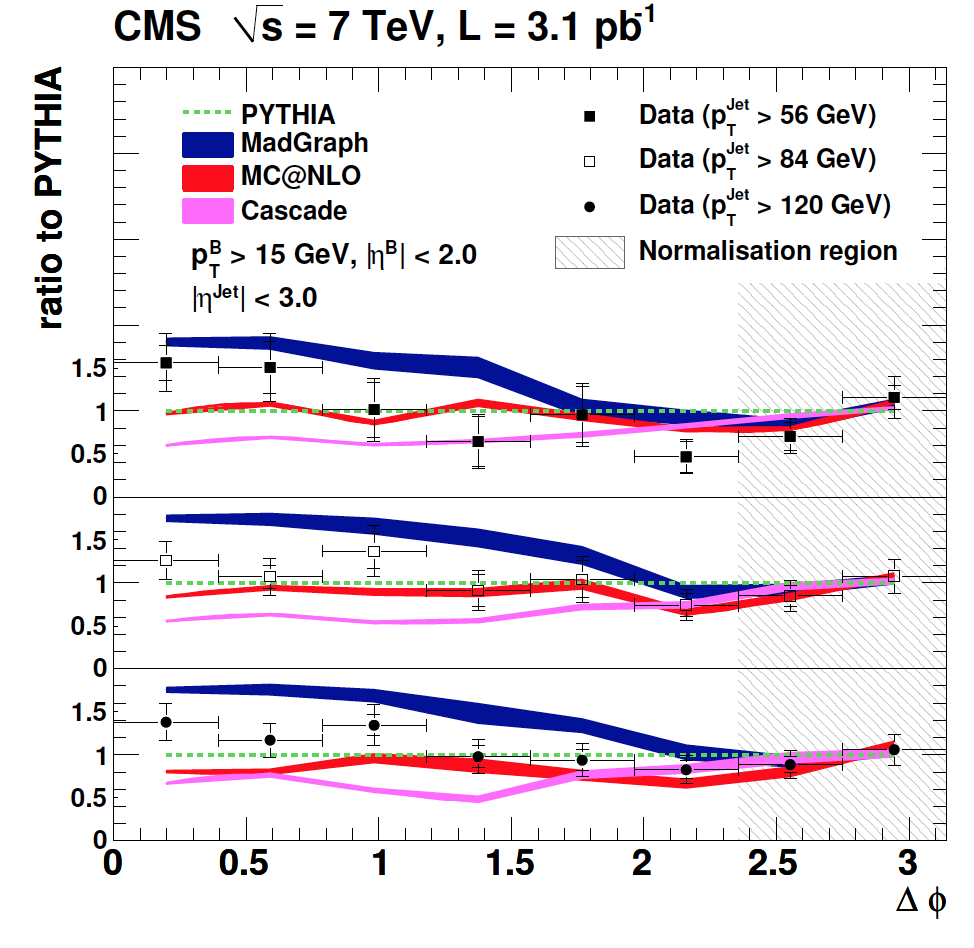
\includegraphics[width=.32\textwidth]{Plots/BBbarCMS7TeV}
\caption{(Left) $\Dzero$ production cross sections measured by the ALICE experiment at LHC in pp collisions at 7 TeV and by the STAR experiment at RHIC at 200 and 500 GeV. 
(Middle) $\Bplus$ production measured by the ATLAS experiment in pp collisions at 7 TeV. (Right) $\rm B \bar{B}$ azimuthal correlation measured by the CMS experiment in pp collisions at 7 TeV.}
\label{fig:ppresults}     
\end{figure}


\section{Proton-nucleus measurements}
\label{pAmeasurements}
In presence of a nuclear environment, the yield of production of light and heavy particles can be modified in absence of any deconfined medium. In particular, modifications of the 
parton distribution functions (PDFs) in the nucleus with respect to nucleon PDFs (e.g. due to shadowing) are expected to be responsable for sizeable modifications of the heavy-flavour cross section at 
low transverse momenta. In order to quantify the effects of these phenomena and validate the hypothesis that the suppression observed in nucleus-nucleus collisions is a consequence of the presence of a a hot and dense medium, 
one can study the heavy-flavour production in proton-nucleus collisions, where the formation of the Quark-Gluon Plasma is not expected. In the last years, the role of ``reference'' of proton-nucleus measurements have been deeply questioned. 
However, at the present moment, no measurement has highlighted the presence of sizeable jet quenching phenomena in proton-nucleus or proton-proton collisions, suggesting that measurements of production yields in smaller 
collision systems can still be used to isolate the effect of cold nuclear matter effects.
The nuclear modification factors $\rpa$ of heavy-flavoured particles have been measured both at RHIC and at the LHC. Thanks to the very high statistics 2016 pPb run, the $\rpa$ of $\Dzero$
mesons have been measured at the LHC with very high precision (Fig.~\ref{fig:RpA}). The measurements performed by LHCb at forward and backword rapidity have highlighted for the first time significant modifications of the production 
yields of D mesons for $\pt<$10 GeV in pPb collisions, which are compatible with the predictions of models that include the effect of modifications of nuclear PDFs. 
The measurement performed by ALICE at central rapidity and an a simple rapidity extrapolation of the LHCb measurement 
show that at central rapidity the effect of cold nuclar matter effects at low $\pt$ is smaller or equal to about 15$\%$. At higher $\pt$, as expected, no significant deviations
from binary scaling ($\rpa$=1) was observed.  In the beauty sector at the LHC, measurements of heavy-flavour electrons performed by ALICE and exclusive B-meson measurements from CMS have measured $\rpa$ consistent with 
unity from 1 to 60 \GeVc at mid rapidity with uncertainties of about 30-40$\%$. A recent CMS measurement of the non-prompt $J/\Psi$ $\rpa$ has measured at central rapidity $\rpa$=1 with uncertainty smaller than 15$\%$. 
A new impressive LHCb measurement of non-prompt $J/\Psi$ $\rpa$ performed down to 0 \GeVc has highlighted for the first time a significant deviation from unity for the $\rpa$ at forward rapidity as expected in 
presence of nuclear shadowing also in the beauty sector. Also at the RHIC energies, the $\rpa$ of beauty has been recently measured via the reconstruction of non-prompt $J/\Psi$ decays. 
The PHENIX collaboration measured a $\rpa$ consistent with unity with uncertainties of the order of 40--50$\%$.
\begin{figure}[ht]
\centering
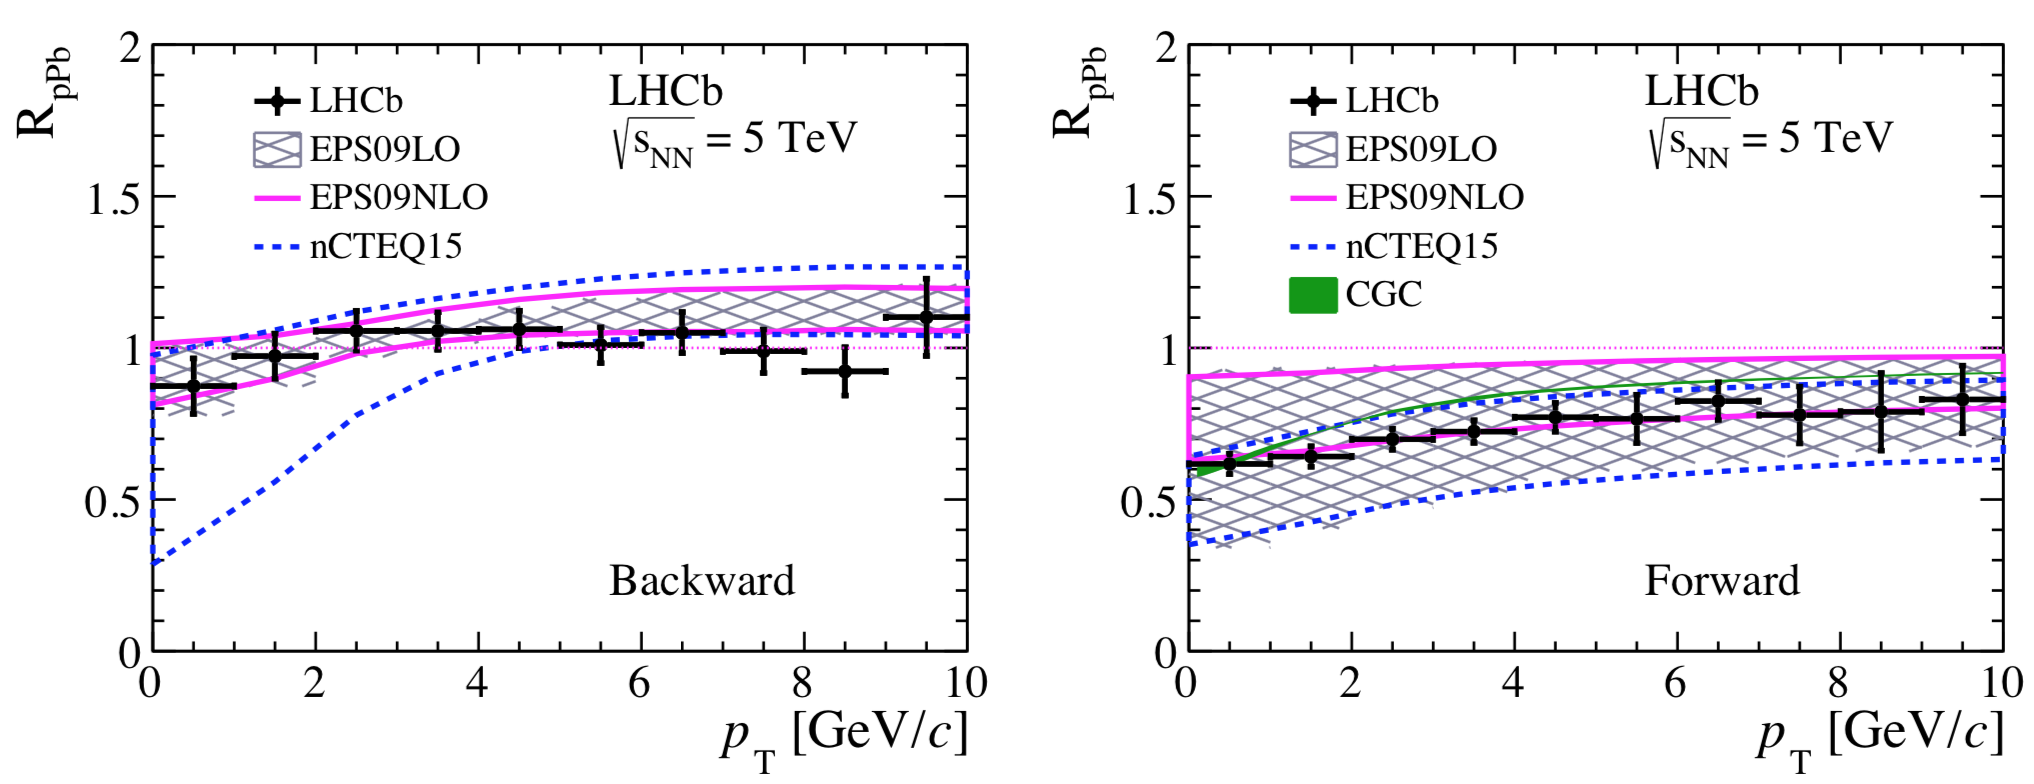
\includegraphics[width=.65\textwidth]{Plots/DRpAvsptLHCb2017}
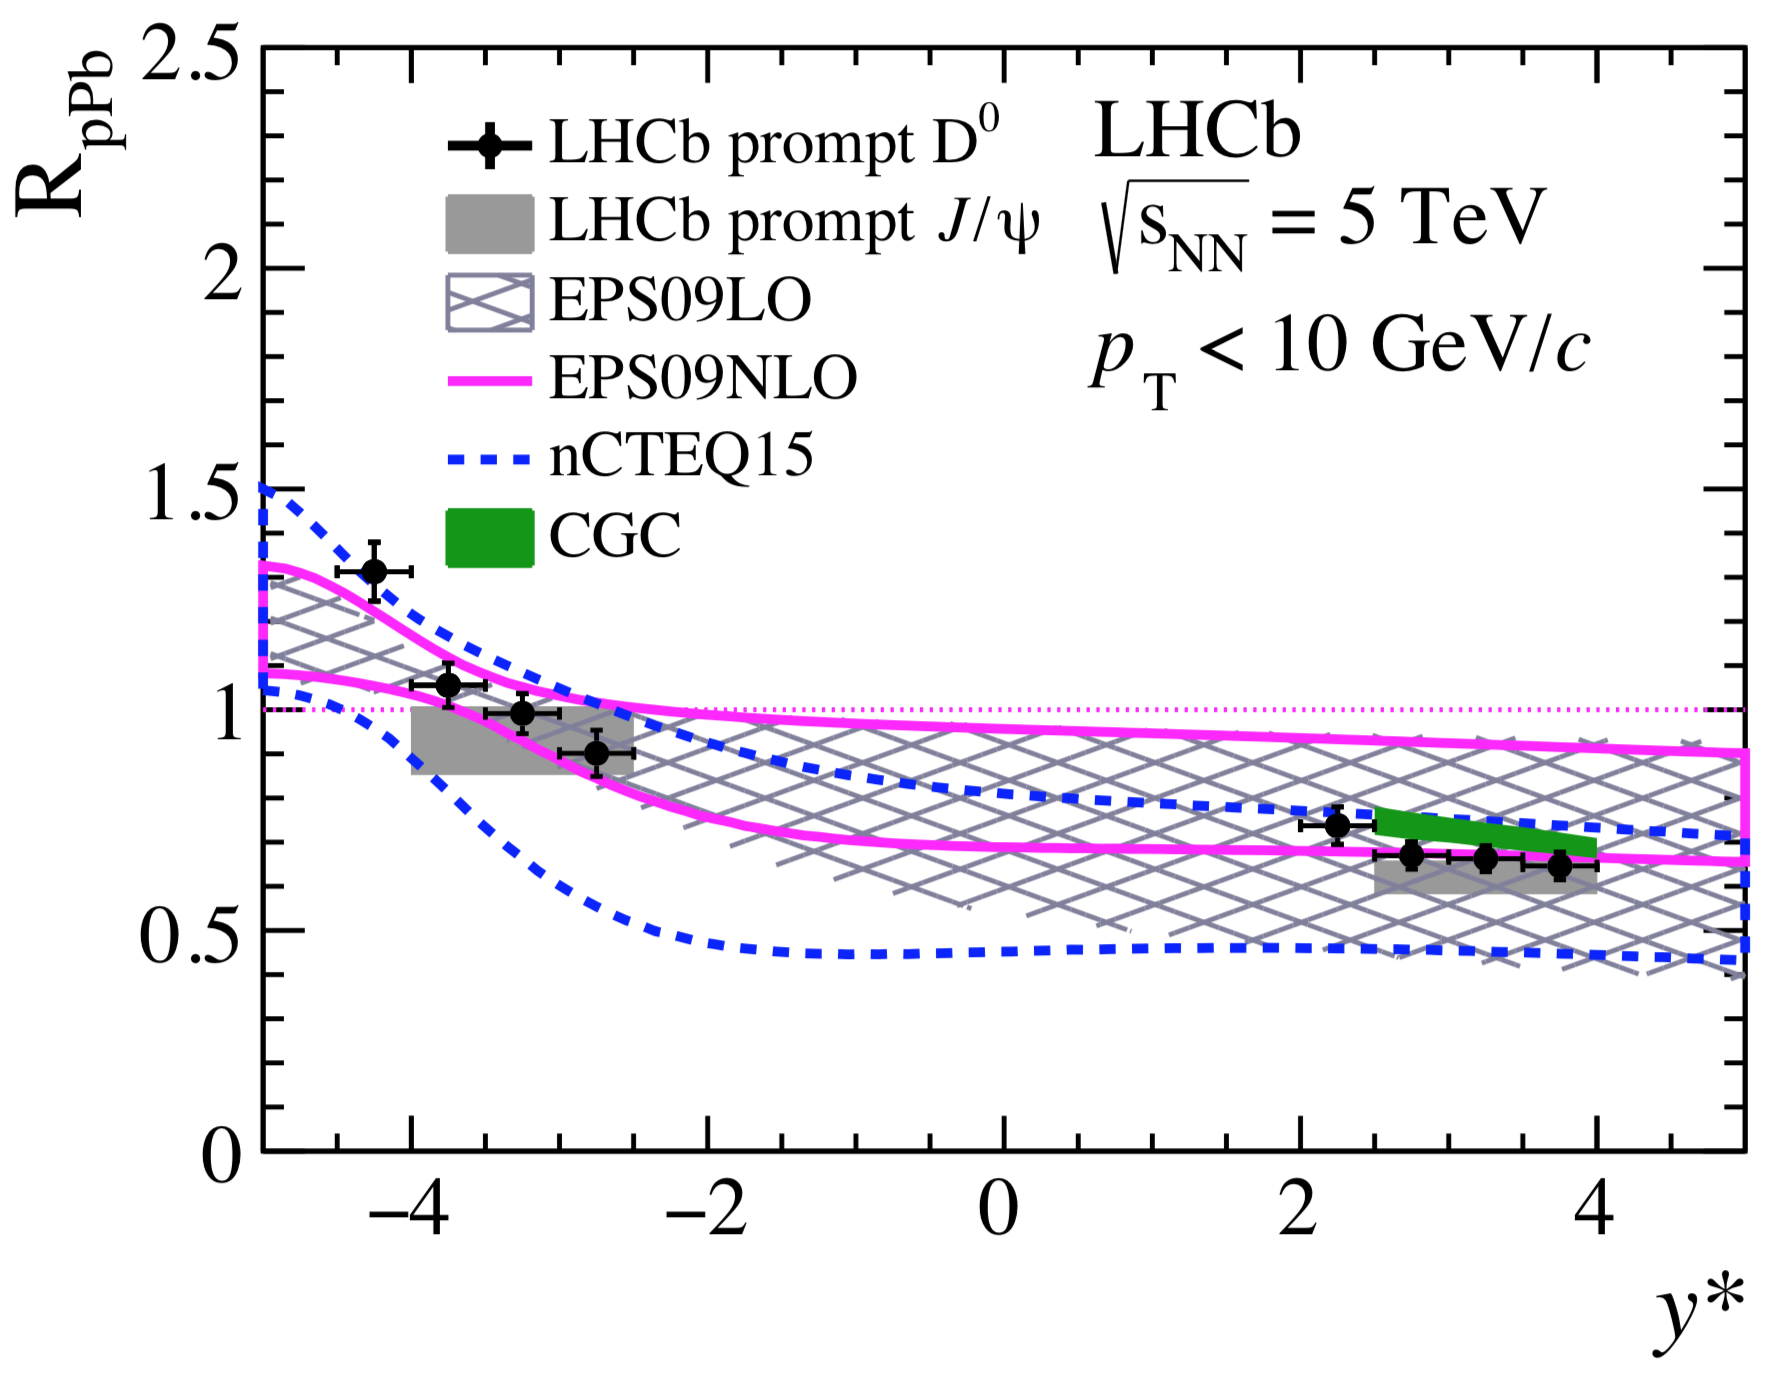
\includegraphics[width=.32\textwidth]{Plots/DRpALHCb2017}
%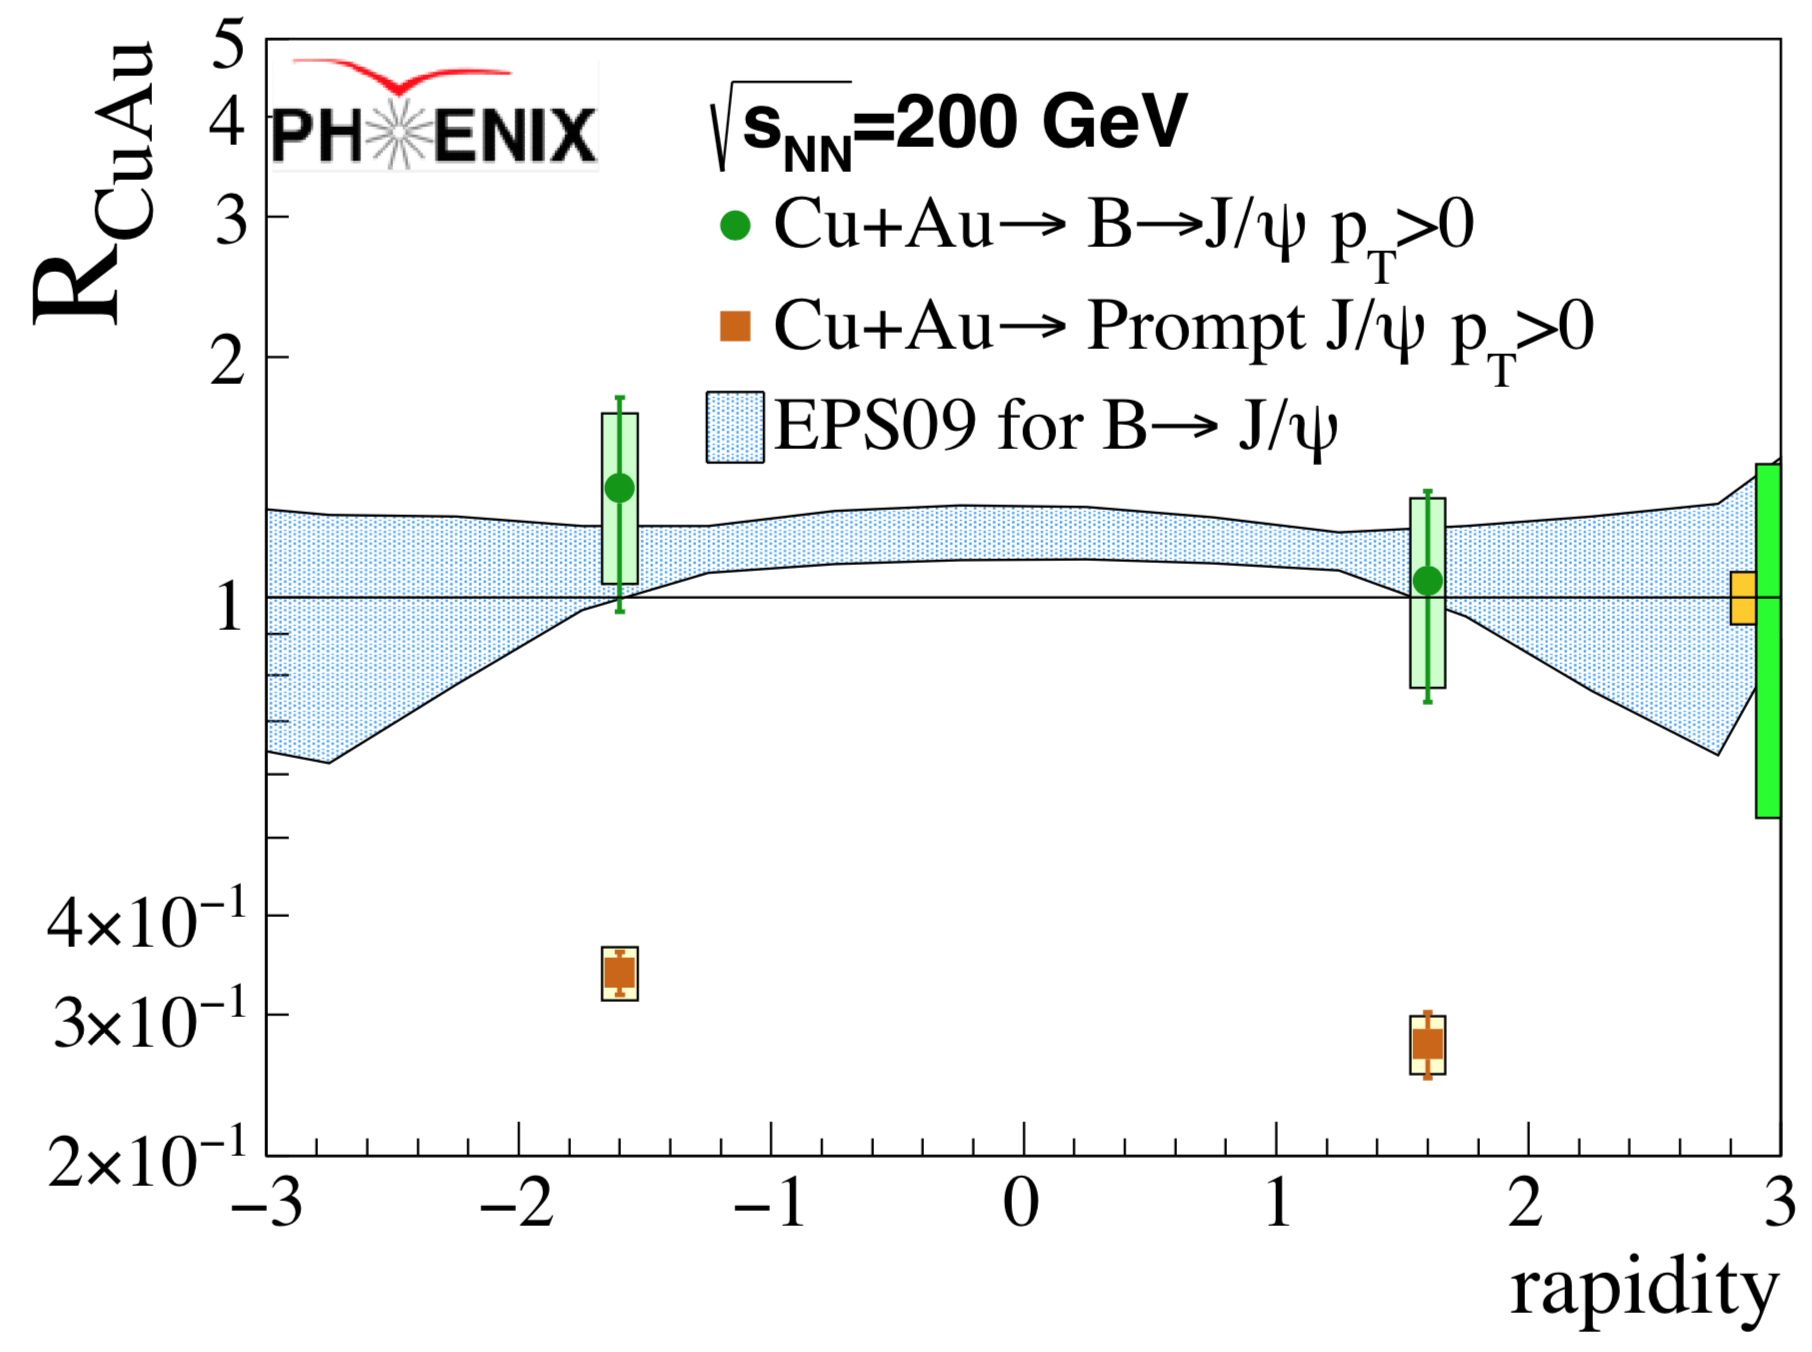
\includegraphics[width=.45\textwidth]{Plots/BRpAPHENIX}
\caption{$\Dzero$ $\rpa$ in the backward (left) and forward (right) rapidity as a function of $\pt$ and as a function of rapidity for $\pt<$10 \GeVc measured by the LHCb collaboration in pp collisions at 7 TeV.}
\label{fig:RpA}     
\end{figure}


\section{Nucleus-nucleus measurements}
\label{AAmeasurements}
\footnotetext{Biased opionion of the author.}
Evidences of a strong charm suppression at the LHC are observed by the ALICE and the CMS Collaboration using the $\raa$
of promptly produced D mesons at mid-rapidity at a nucleon-nucleon centre-of-mass energy $\sqrtsNN=2.76$ and $\sqrtsNN=5.02$ TeV. 
The two results are fully consistent if compared in the same $\pt$ and centrality region. The \raa of $\Dzero$ mesons at the LHC shows a maximum suppression of 
a factor 5--6 with respect to the pp reference for the 10\% most central collisions in the $\pt$ range of 6--10\GeVc. For $\Dzero$ mesons in the high-$\pt$ range of 60--100\GeVc, a significantly smaller suppression is observed. 
The \raa as a function of $\pt$ is quite well described by several theoretical calculations that include collisional or radiative energy loss or a mixture of the two mechanisms. 
An increasing suppression is observed as a function of centrality as expected in case of the creation of a denser and hotter medium in central PbPb collisions. This trend is also 
well described by theoretical calculations. At RHIC energies, the \raa was also measured by the STAR Collaboration. Quite surprisingly, the \raa of $\Dzero$ mesons was found at the LHC to be almost 
completely consistent with the charged particle \raa from 1 to 100 \GeVc. As discussed several times in several occasions, the same \raa in presence of very different (and steeply falling) $\pt$-spectra and fragmentation 
functions does not imply the same energy loss. On the contrary, the evidence of a very similar suppression for charged particles and D mesons seems to be a very fortunate (too fortunate?) cancellation of the effects
of different energy loss, $\pt$-spectra and fragmentation functions. Although described by several theoretical calculations, this observation does not present a clear and immediate physics interpretation\footnotemark[\value{footnote}].
At RHIC, on the contrary, the D-meson and the charged particle $\raa$ show a very significant discrepancy for $\pt<$2 \GeVc.  The D-meson $\raa$ shows indeed values larger than 1.5 even if with large uncertaintes. 
Such a big difference between the ratio of the light and D-meson \raa at the two energies could be due to several effects like differences in radial flow or in nuclear PDF modifications at the two energies, 
even if explanining a difference of a factor 3 with these effects seems quite challenging\footnotemark[\value{footnote}]. 

\begin{figure}[ht]
\centering
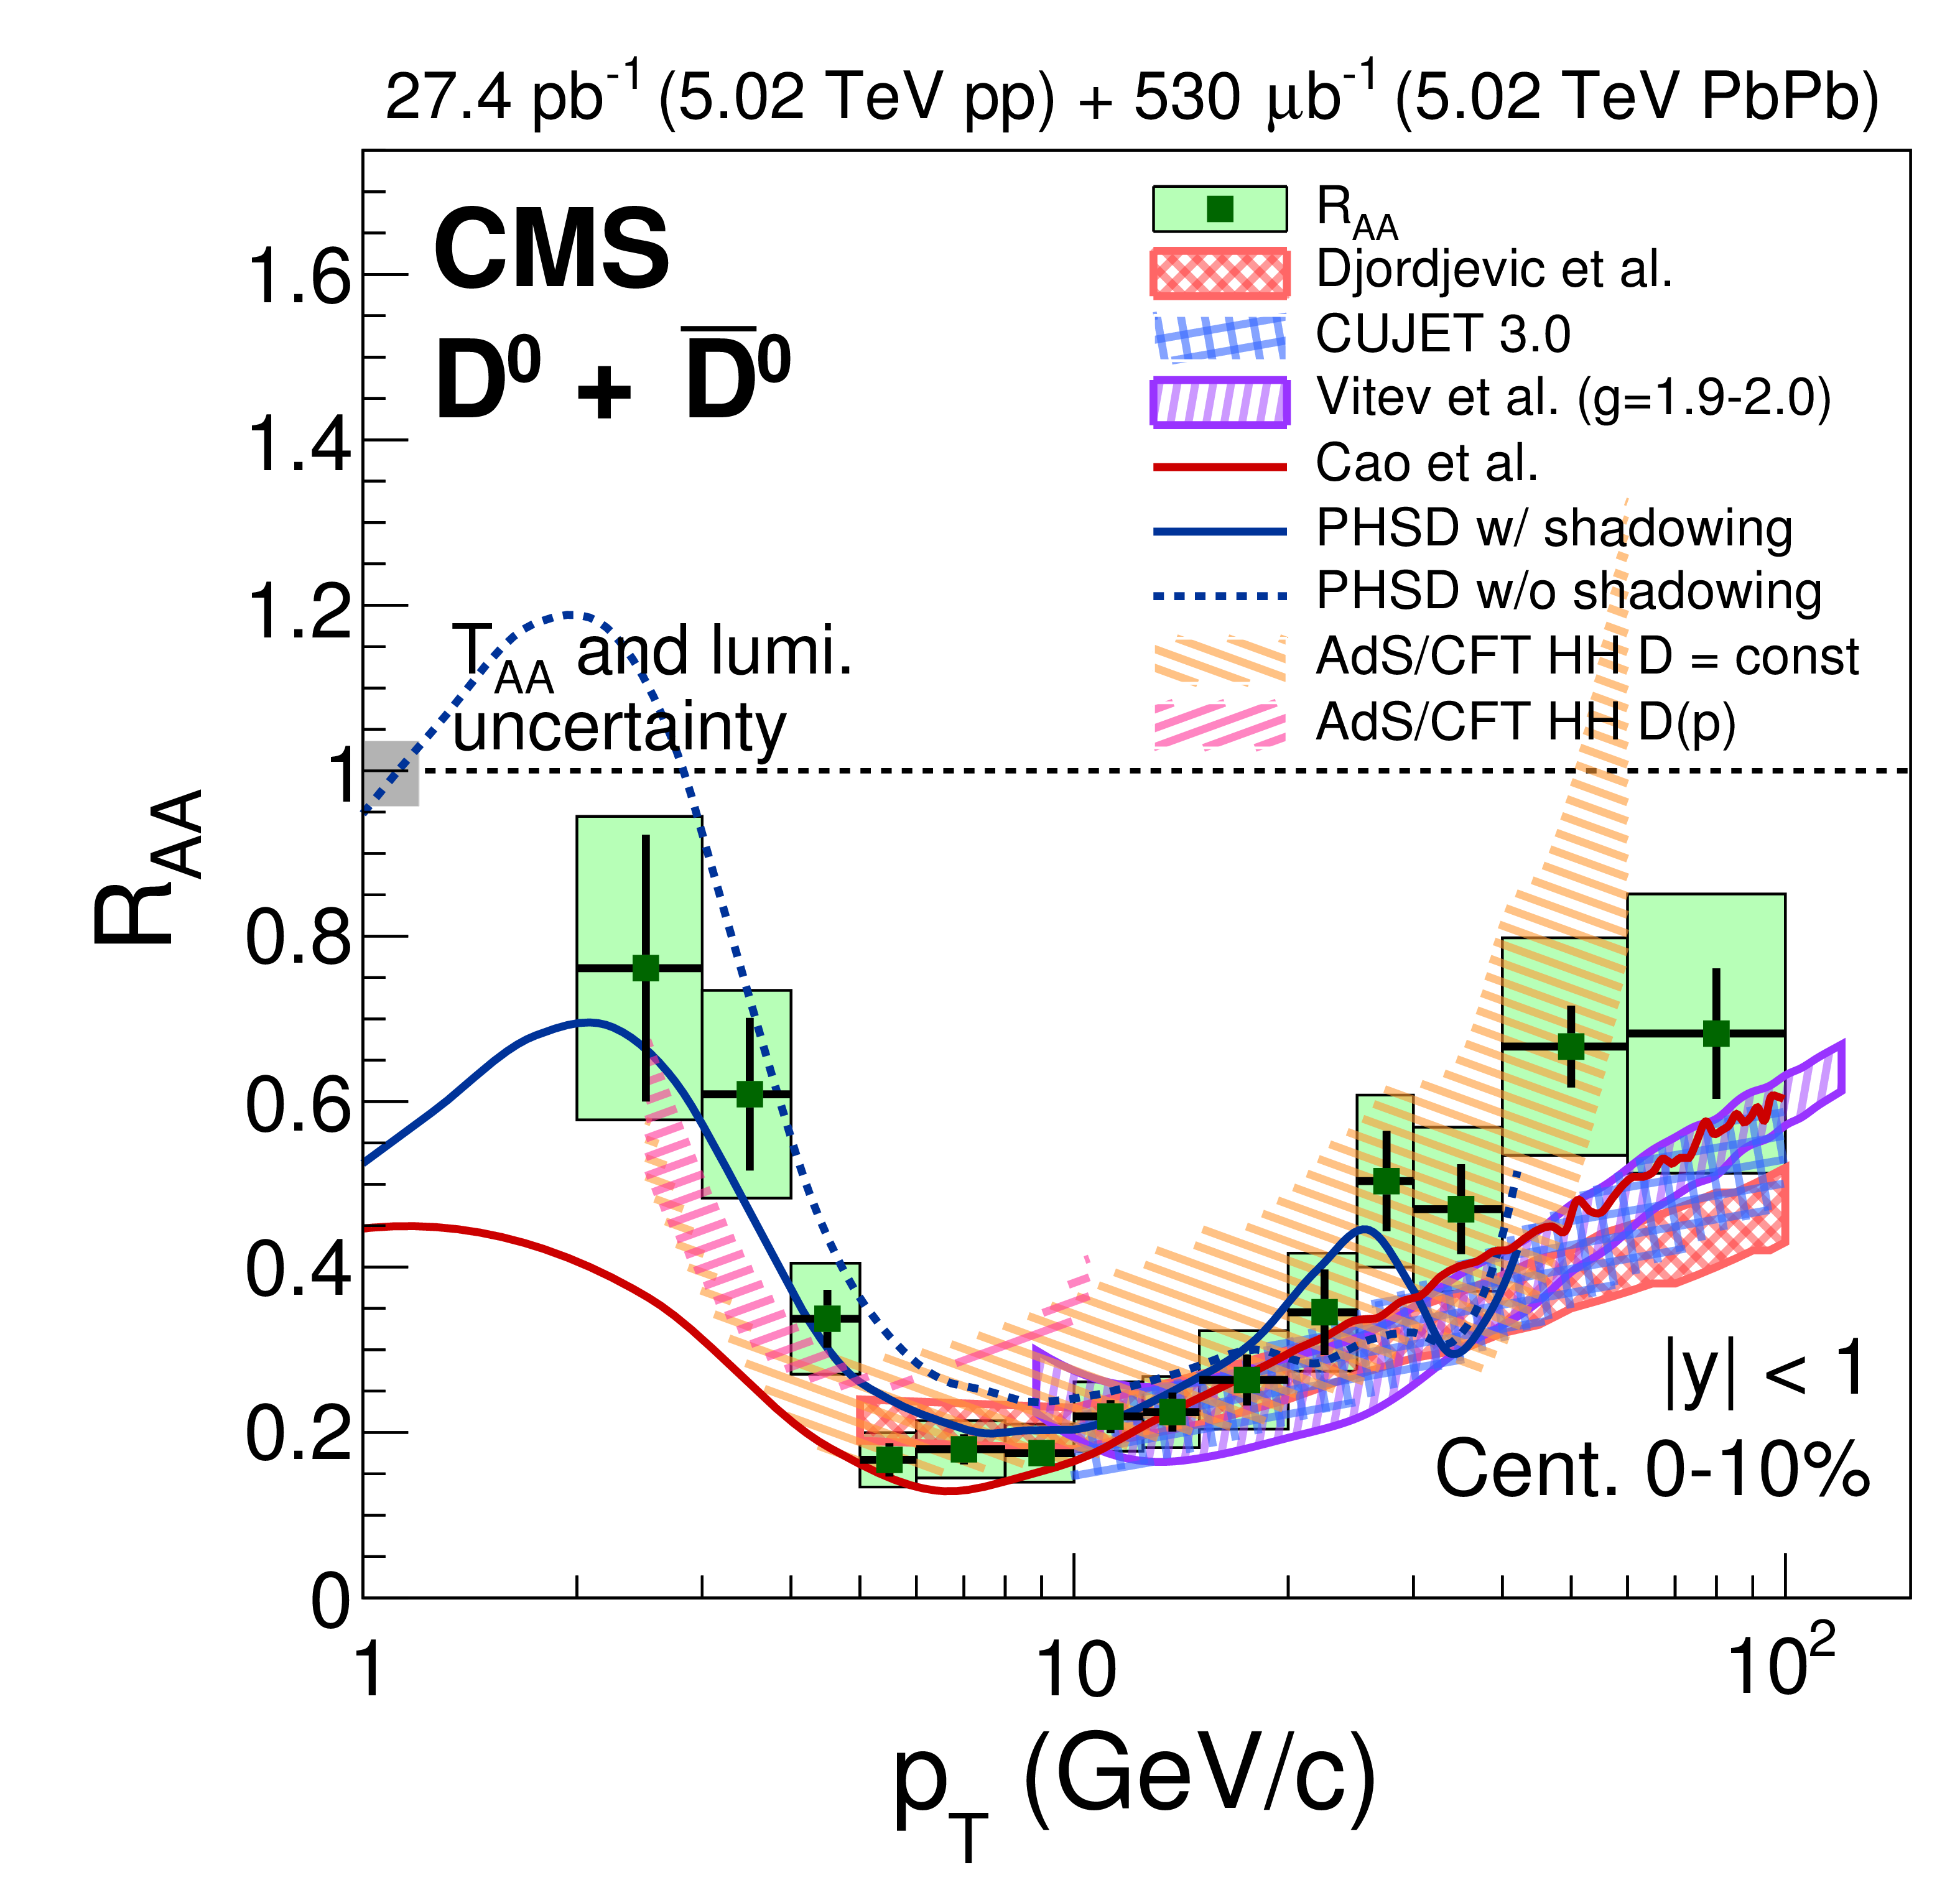
\includegraphics[width=.30\textwidth]{Plots/DRAACMS010}
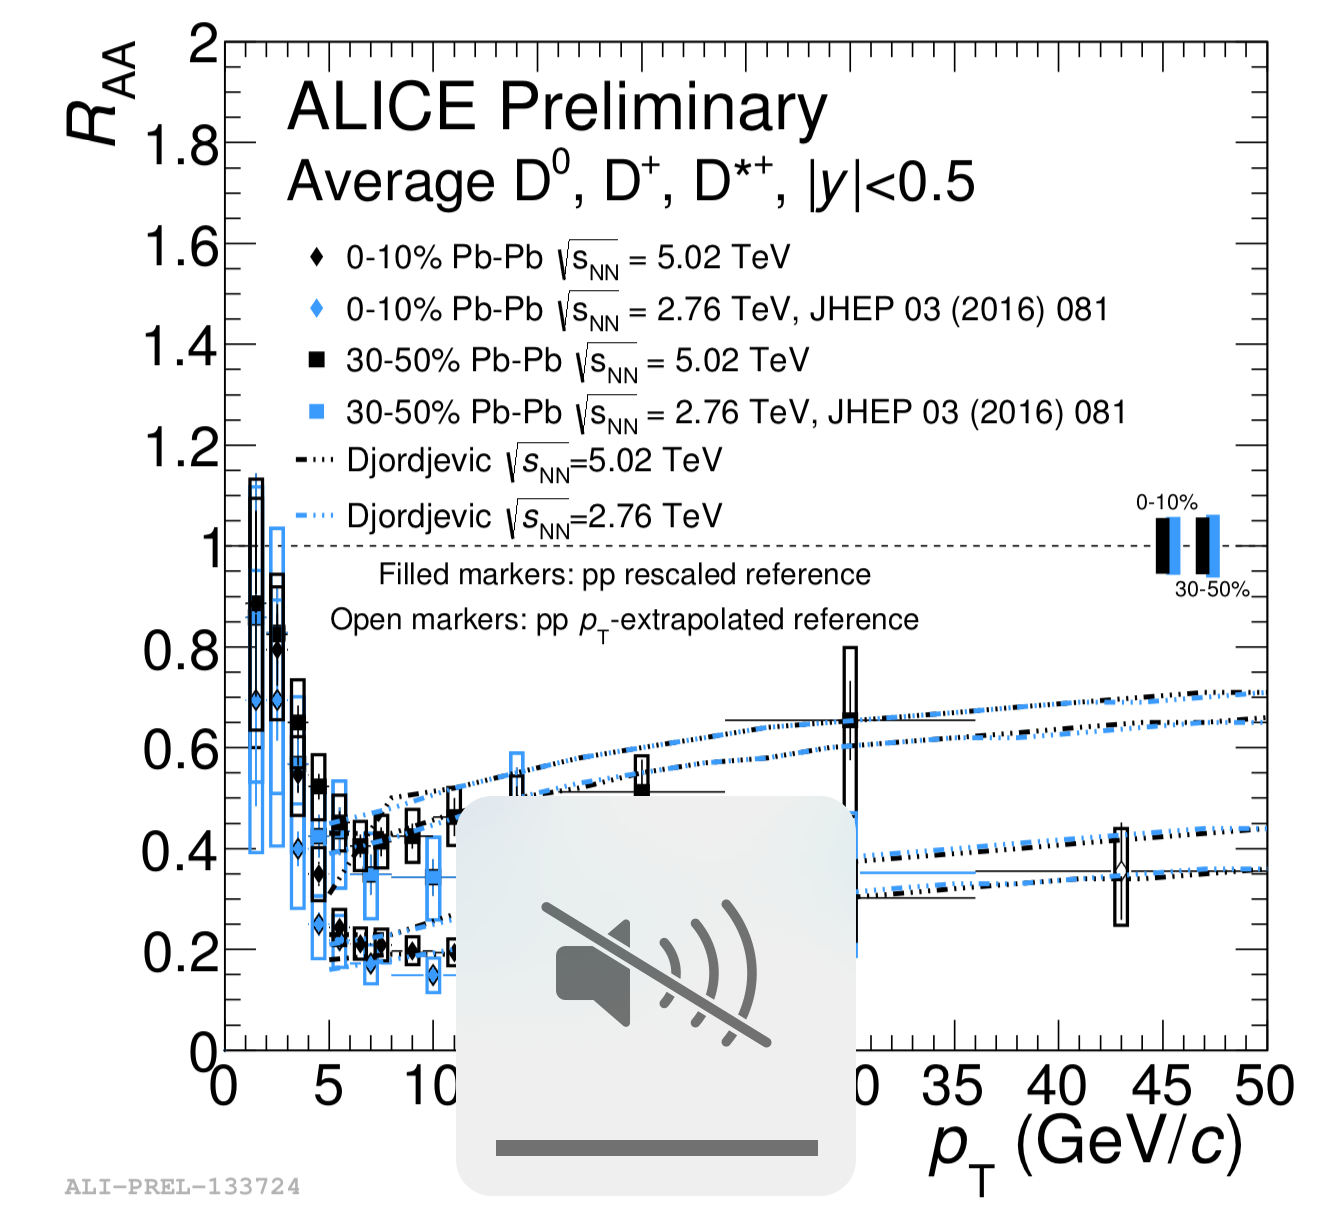
\includegraphics[width=.30\textwidth]{Plots/DRAAALICECentrality502}
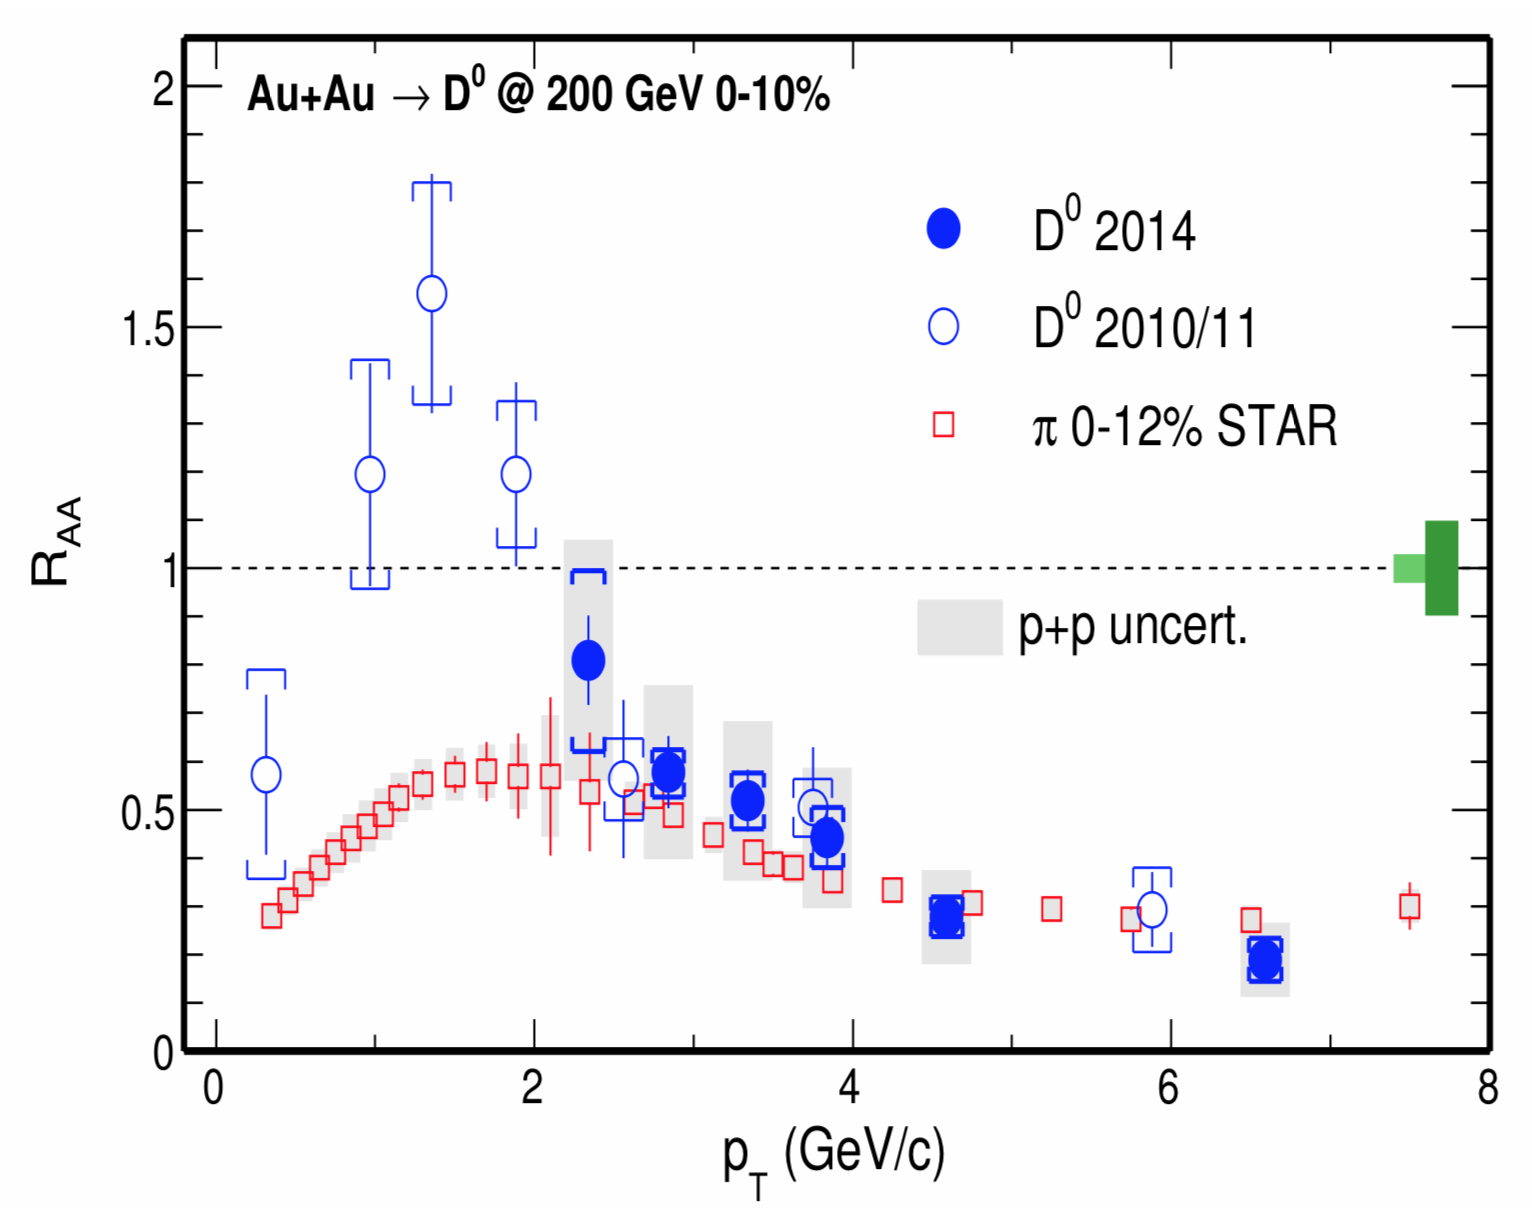
\includegraphics[width=.37\textwidth]{Plots/DRAASTARAuAu}
\caption{Please write your figure caption here}
\label{DRAA}     
\end{figure}

The suppression of beauty particles was also measured by different collaborations both at RHIC and at the LHC. At the LHC, the $\raa$ of beauty 
particles was measured down to about 2 GeV by the ALICE experiment with heavy-flavour electron measurements and from 3 GeV up to 50 GeV 
using exclusively reconstructed B mesons and non-prompt B meson decays ($\bdecayX$). As shown in the left panel Fig.~\ref{fig:FlavourRAA}, 
the current measurements indicate a hint of different suppression of beauty and charmed particles at low-intermediate $\pt$ that vanishes when 
going at higher transverse momenta. Several (very reasonable) concerns were raised in several discussion with respect to the CMS comparison plot. 
In the next few lines, I would try to report the current, personal understanding of the author. 
The first is related to the fact that in this plot the $\pt$ of the non-prompt J/$\Psi$ is not corrected for the difference between the $\pt$ of the beauty 
hadron and the $\pt$ of the non-prompt J/$\Psi$. This is indeed a valid point that should be addressed in future version of this plot expecially for 
what concerns the low-$\pt$ region. For the higher-$\pt$, the fact that the $\raa$ does not show a strong $\pt$-dependence should make this 
missing correction less relevant. The second concerns is related to the possible discrepancy between the non-prompt J/$\Psi$  and the exclusive B result. 
In this case, I would stress the fact that the uncertainties on the current B-meson $\raa$ are quite sizeable and the two measurements are still compatible 
within the uncertainties. However, a proper statistical study that accounts for the bin-by-bin correlation of the uncertainties should be performed 
after correcting for the non-prompt J/$\Psi$ shift discussed above. The last concerns is related to the fact that the results reported here mix measurements 
performed in different rapidity regions. Also in this case, the comment is well posed and a proper answer would require more differential analysis of 
the $\raa$ of the different species as a function of rapidity or at least the measurement of the different species in the exact same rapidity region\footnote{The reason for which this was currenlty not still done
is related to the fact that the a B-meson measurement in a smaller rapidity region is currently not possible due to the limited statistics and the non-prompt J/$\Psi$ measurement at central rapidity cannot 
reach the very low-momentum region as a consequence of the kinematic cuts applied to the muons and to the characteristics of the CMS muon detectors.}. 
The recent measurement of non-prompt J/$\Psi$ of CMS as function of the rapidity does not indicate a strong y-dependence of the suppression. This evident 
seem to indicate that the different y-dependence of the measurements should not affect too dramatically the physics conclusions we draw with the current version 
of this plot. 

\begin{figure}[ht]
\centering
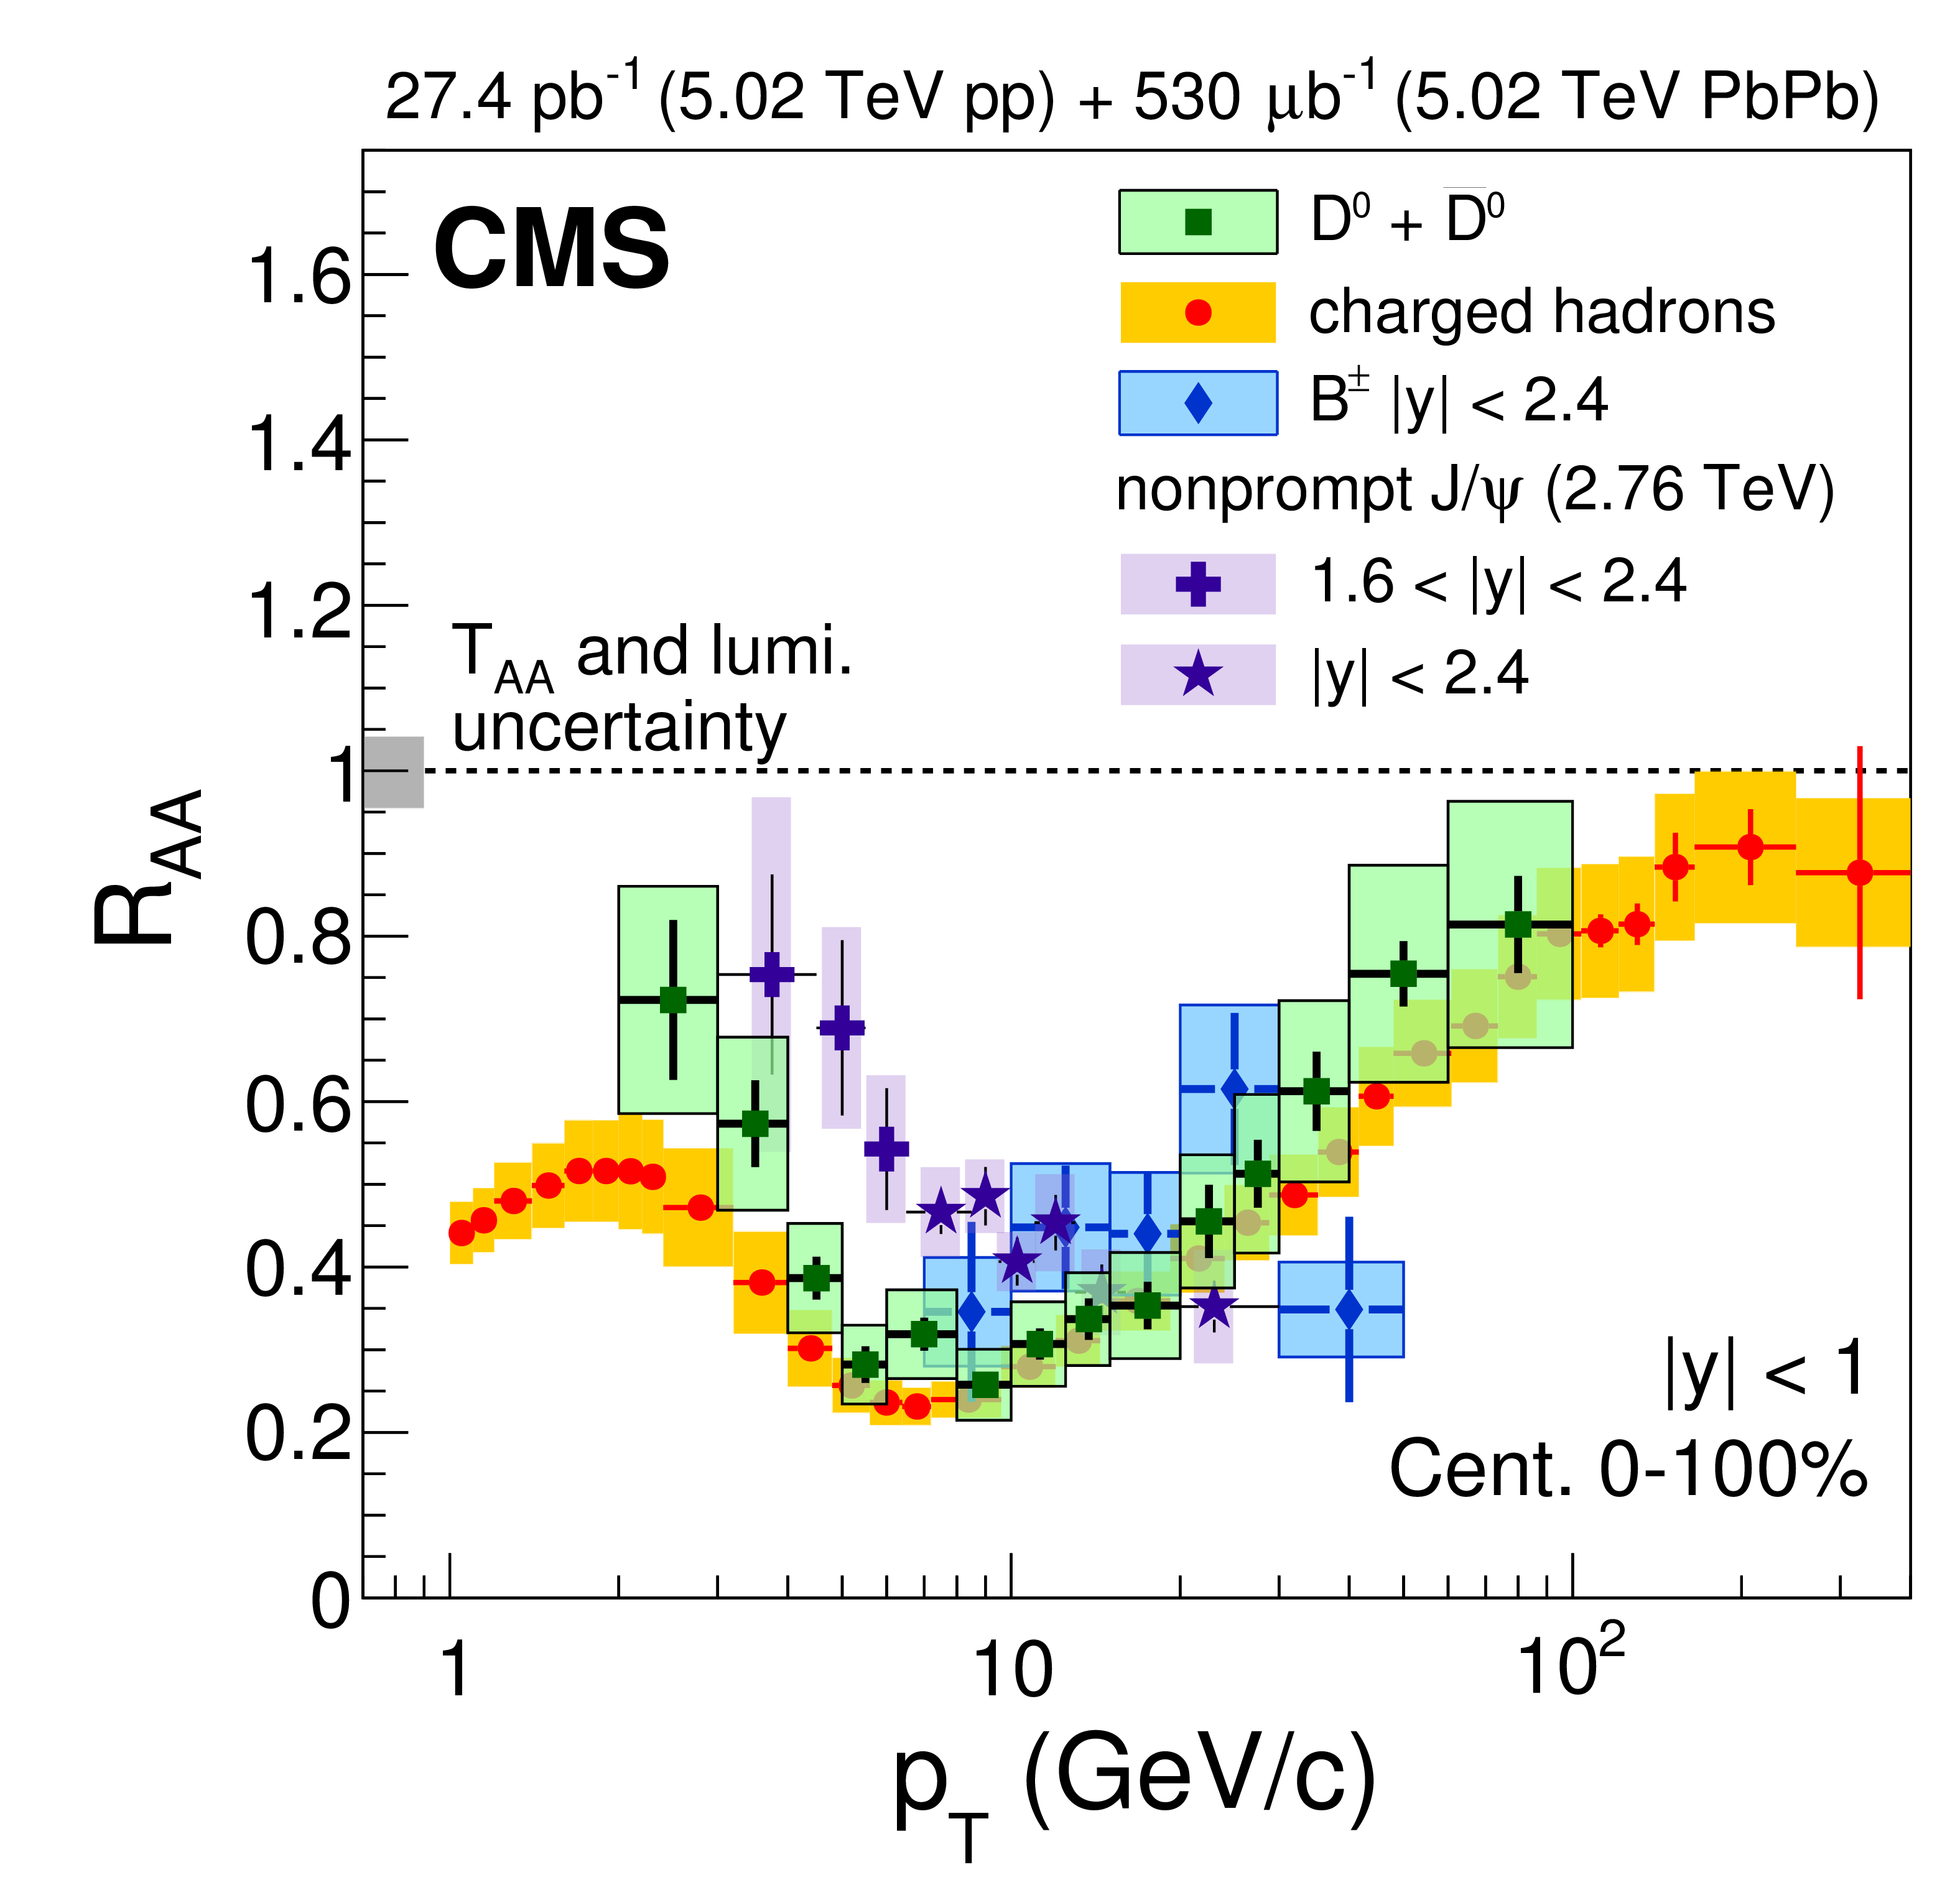
\includegraphics[width=.32\textwidth]{Plots/DBNonPromptRAACMS}
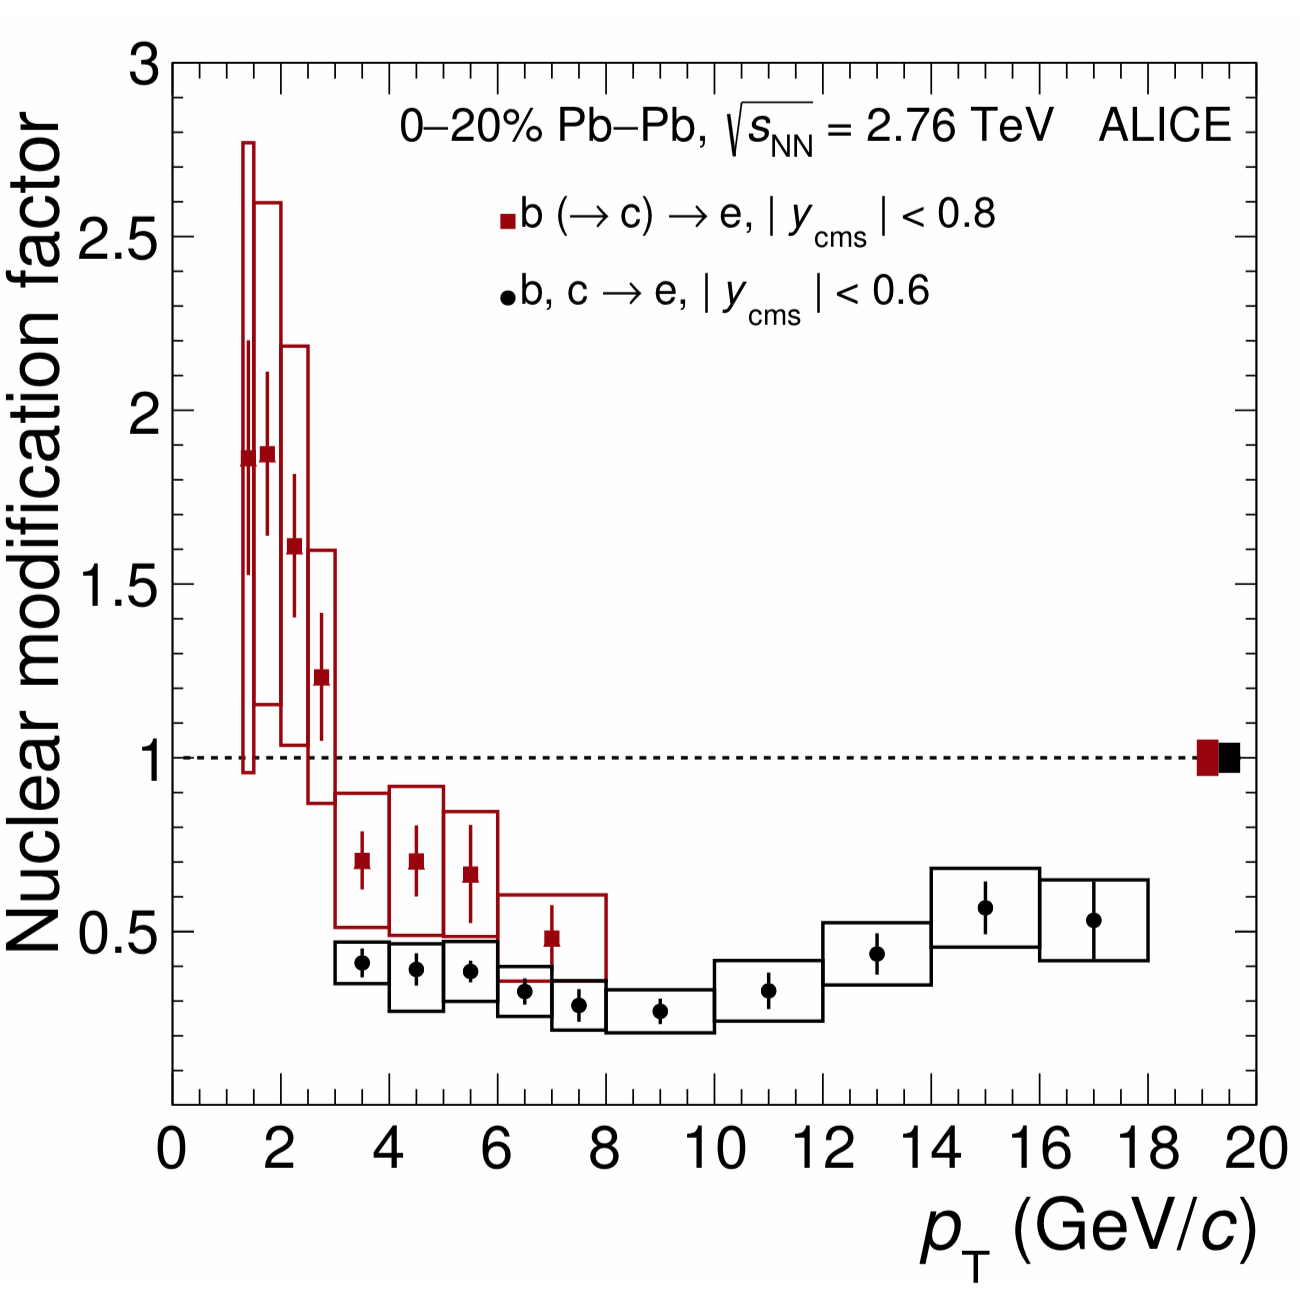
\includegraphics[width=.32\textwidth]{Plots/HFelectronsALICE}
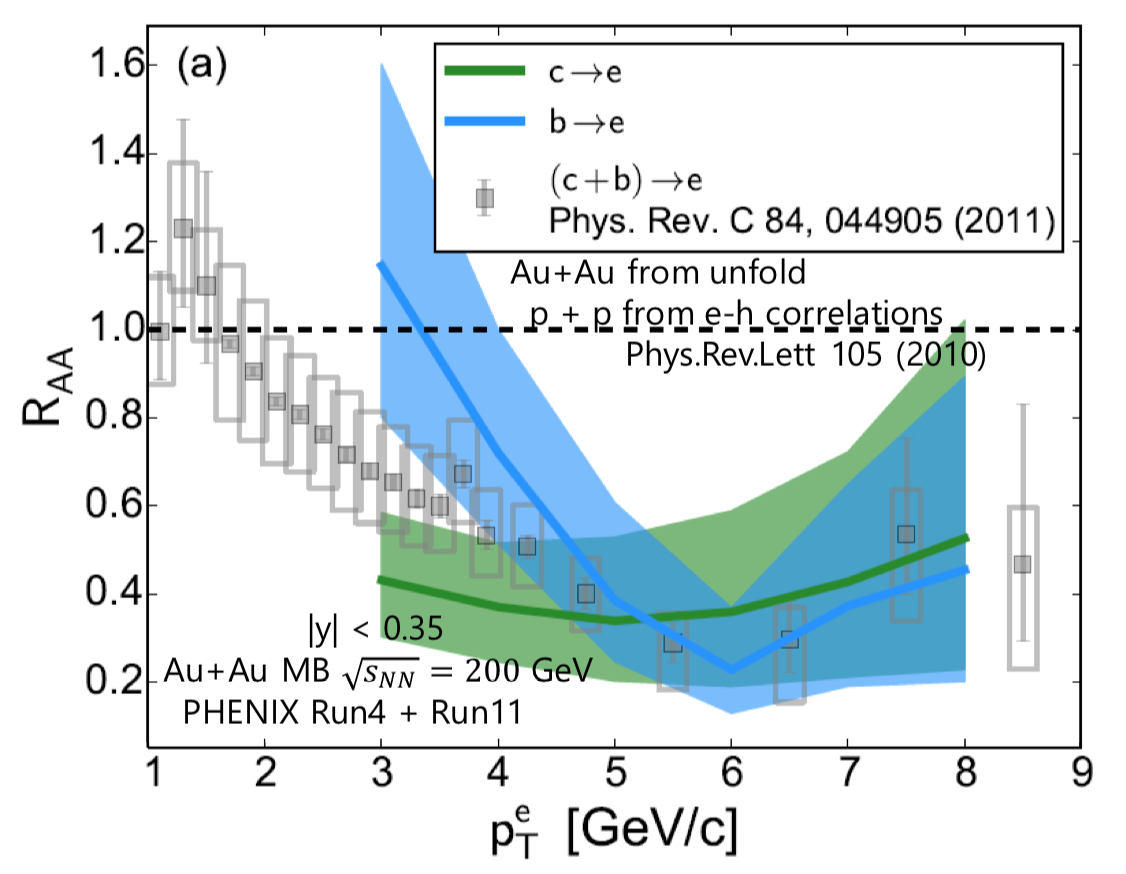
\includegraphics[width=.32\textwidth]{Plots/BPHENIXAuAu}
\caption{Please write your figure caption here}
\label{fig:FlavourRAA}     
\end{figure}

A first indication of a relevant contribution of recombination was also found both at RHIC and at the LHC. Indeed a first hint of a larger $\raa$ of $\Ds$ mesons with respect to non-strange 
D mesons was observed both by the ALICE and the STAR collaboration in central and semi-central collisions. This is currently interpretated as an indication that coalescence is playing 
a relevant role in the hadronisazion of charm quarks in heavy-ion collisions. The observation of this phenomenon seems to confirm the presence of free color charges are present in the medium. 
In absence of color connectivity (the possibility for color charges to ``travel'' inside the medium over large distances) , recombination processes cannot take place. A precise estimation of the effect of 
recombination is also very important as an input for theoretical calculations that describe the suppression of heavy-flavoured particles. A wrong estimation of recombination effects can indeed 
biases our understanding of the magnitude of energy loss processes in heavy-flavour measurements. The STAR Collaboration also recently reported a first measurement of the $\Lambdac$ 
$\raa$ in semi-peripheral gold-gold collisions. Also in this case, an ehnancement with respect to the pp baseline was observed. This result can be intepreted theoretically if we assume that charm 
can recombine in a medium where  di-quark bound states can be formed. 
\begin{figure}[ht]
\centering
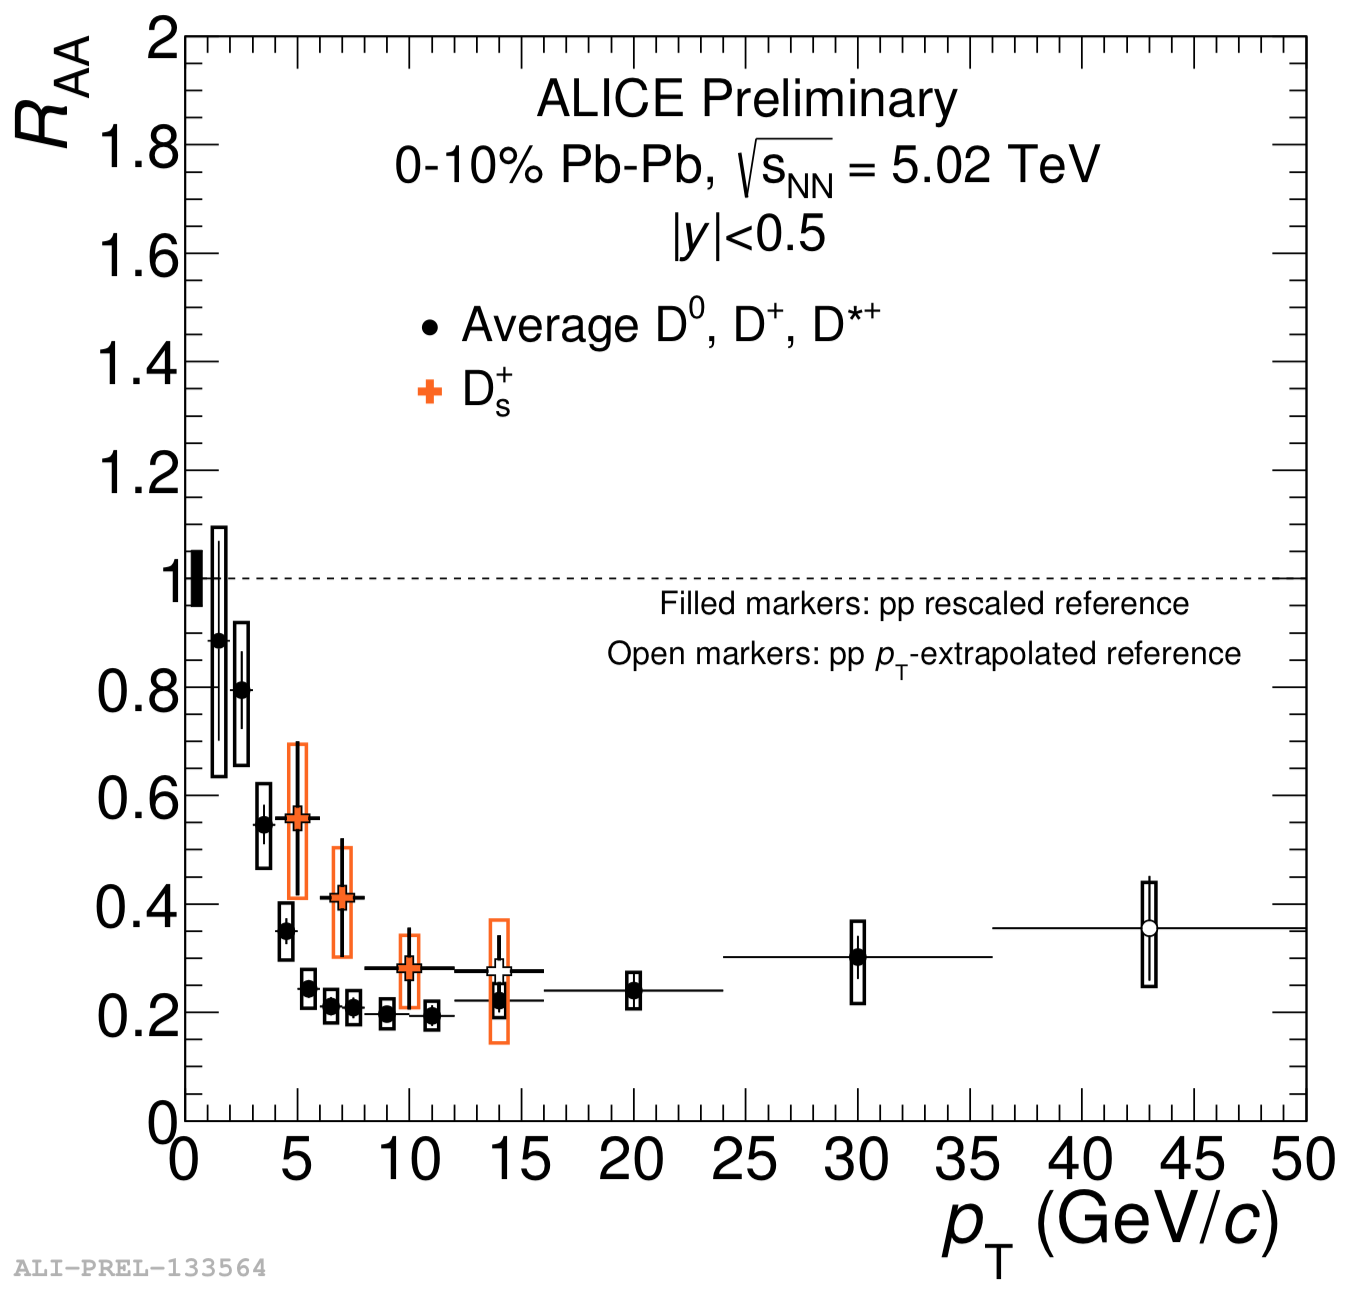
\includegraphics[width=.34\textwidth]{Plots/DsDRAA502TeV}
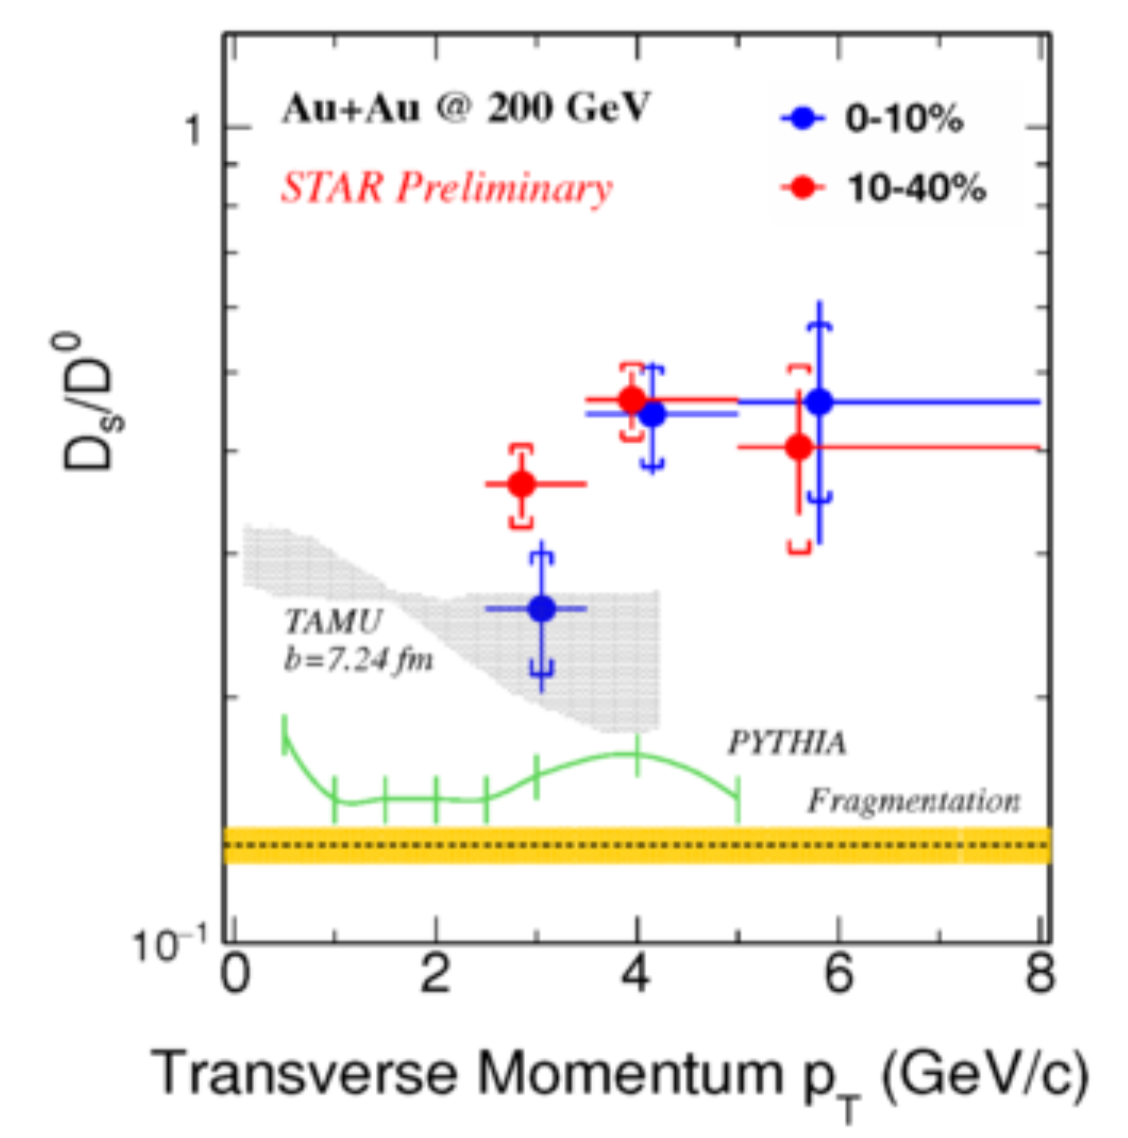
\includegraphics[width=.34\textwidth]{Plots/DsDSTARAuAu}
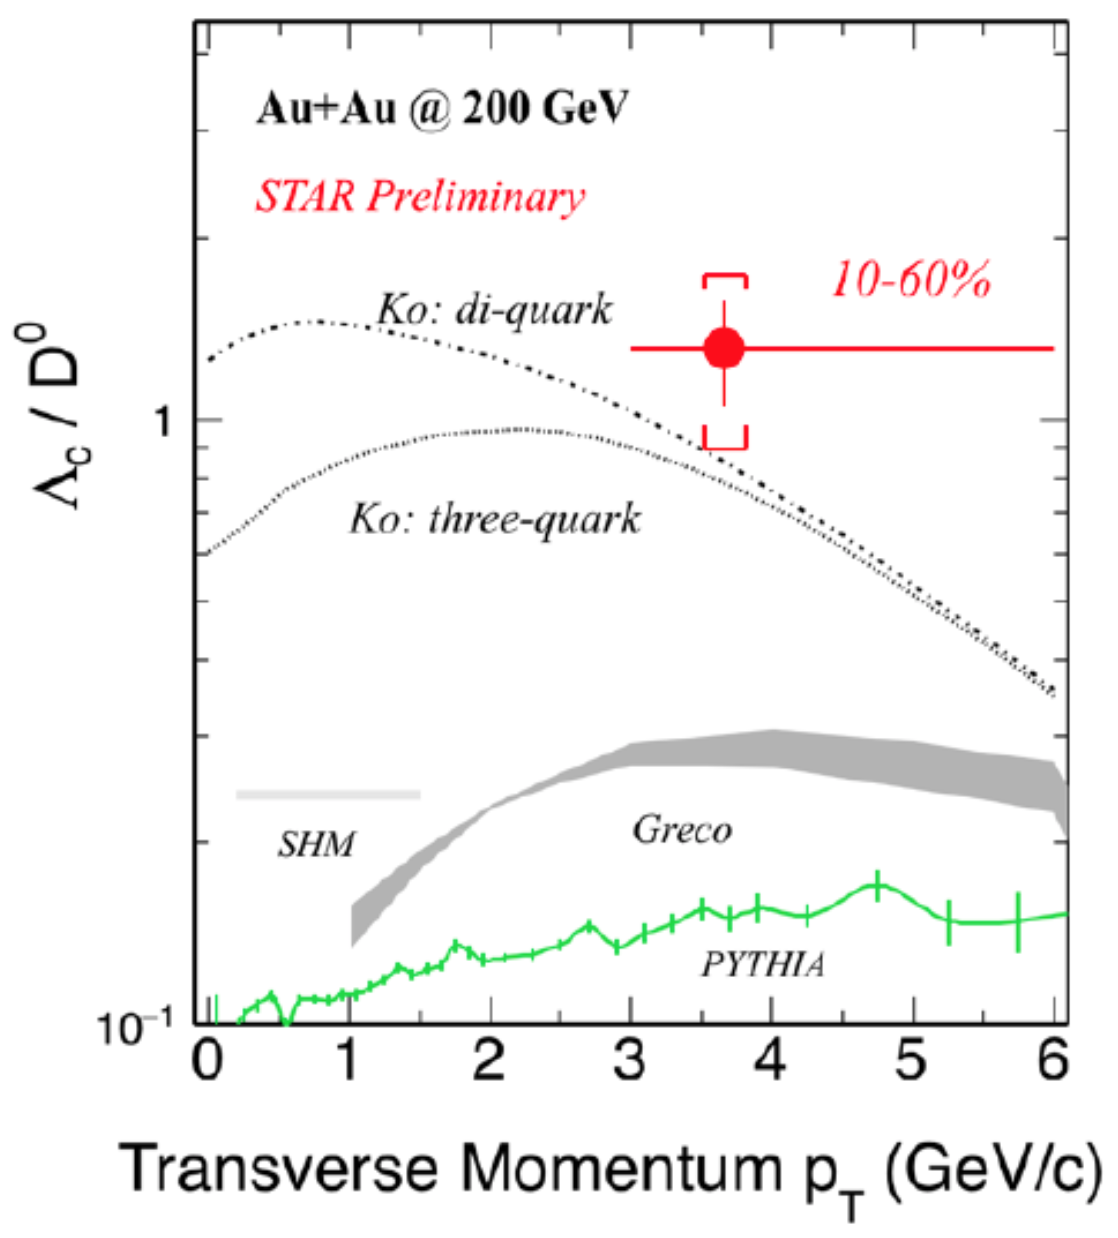
\includegraphics[width=.27\textwidth]{Plots/LambdacRAASTAR}
\caption{Please write your figure caption here}
\label{recombinationMesons}     
\end{figure}

Strong evidences of charm flow were also observed by several collaborations both at RHIC and at the LHC. Large and positive value of the elliptic flow coeffiients $v_{2}$ were measured by ALICE 
and CMS at low-intermediate $\pt$ in semi-pheripheral PbPb collisions and by STAR in AuAu collisions. Due to the limited statistics available at RHIC, the current STAR result is obtained in an integrated 
centrality interval 0--80$\%$. Therefore a direct comparison between the magnitude of the elliptic flow at the two energies cannot be currently done.
At the LHC, where more differential measurement were performed, the magnitude of the D-meson $v_{2}$ coefficient was found to decrease when going from peripheral to more central events as expected 
in case the elliptic flow is generated as a consequence of the initial anysotropy of the fireball.  A non-zero $v_{2}$ is also observed at larger $\pt$ (>10 \GeVc). In this kinematic region, the $v_{2}$ measurement is not 
anymore sensitive to collective phenomena but it is sensitive to in-medium path dependence of energy loss and can be therefore use to contraint jet quenching theoretical calculations. At the LHC, a significant indication 
of smaller $v_{2}$ of D mesons with respect to charged-particle $v_{2}$ was observed. A first hint of non-zero $v_{3}$ of D mesons was also measured by CMS in non-central collisions. 
A complete theoretical interpretation of these results is currently not available. An important theoretical effort is needed 
and it is ongoing to quantify the level of charm thermalisation in the medium, to understand if charm quarks can be described by a hydro-dynamic description 
and to extract the difficusion parameters of charm quarks in the medium using these very precise measurements. At the LHC, a first attempt was made by the CMS collaboration to measure the 
$v_{2}$  coefficient of beauty by the measurement of non-prompt J/$\Psi$ in semi-peripheral PbPb events. The current results, even if still not conclusive, represent a very promising field 
of investigation for future high-luminosity runs. 
\begin{figure}[ht]
\centering
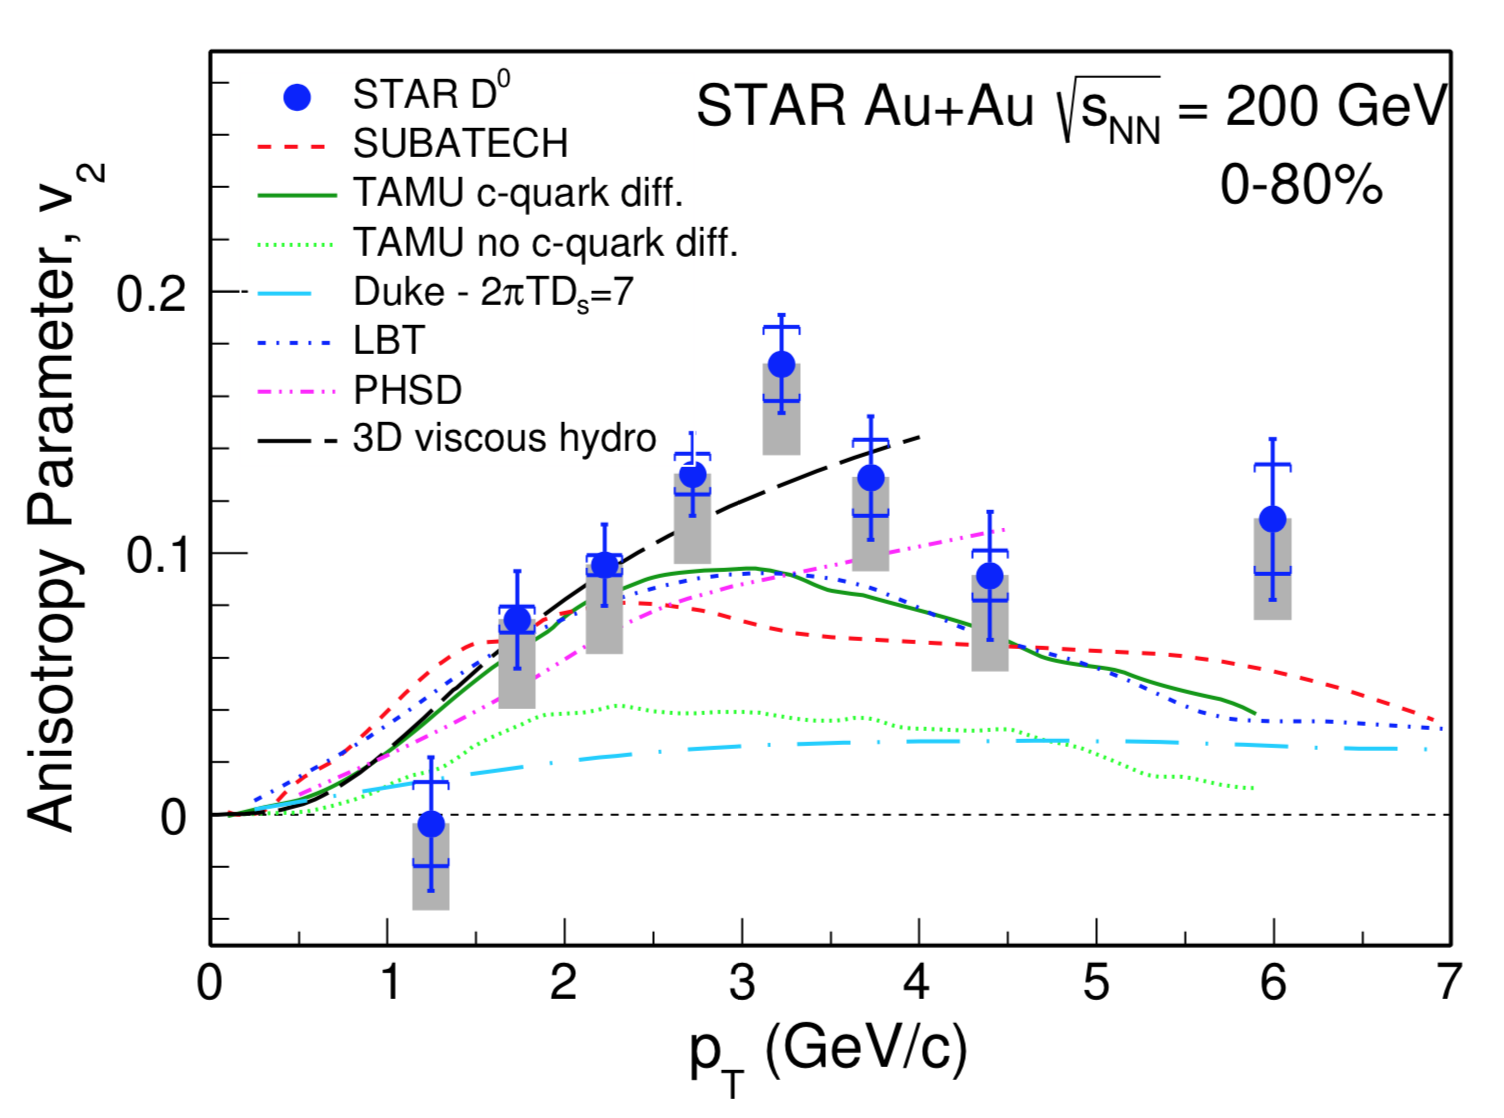
\includegraphics[width=.32\textwidth]{Plots/Dmesonv2STAR}
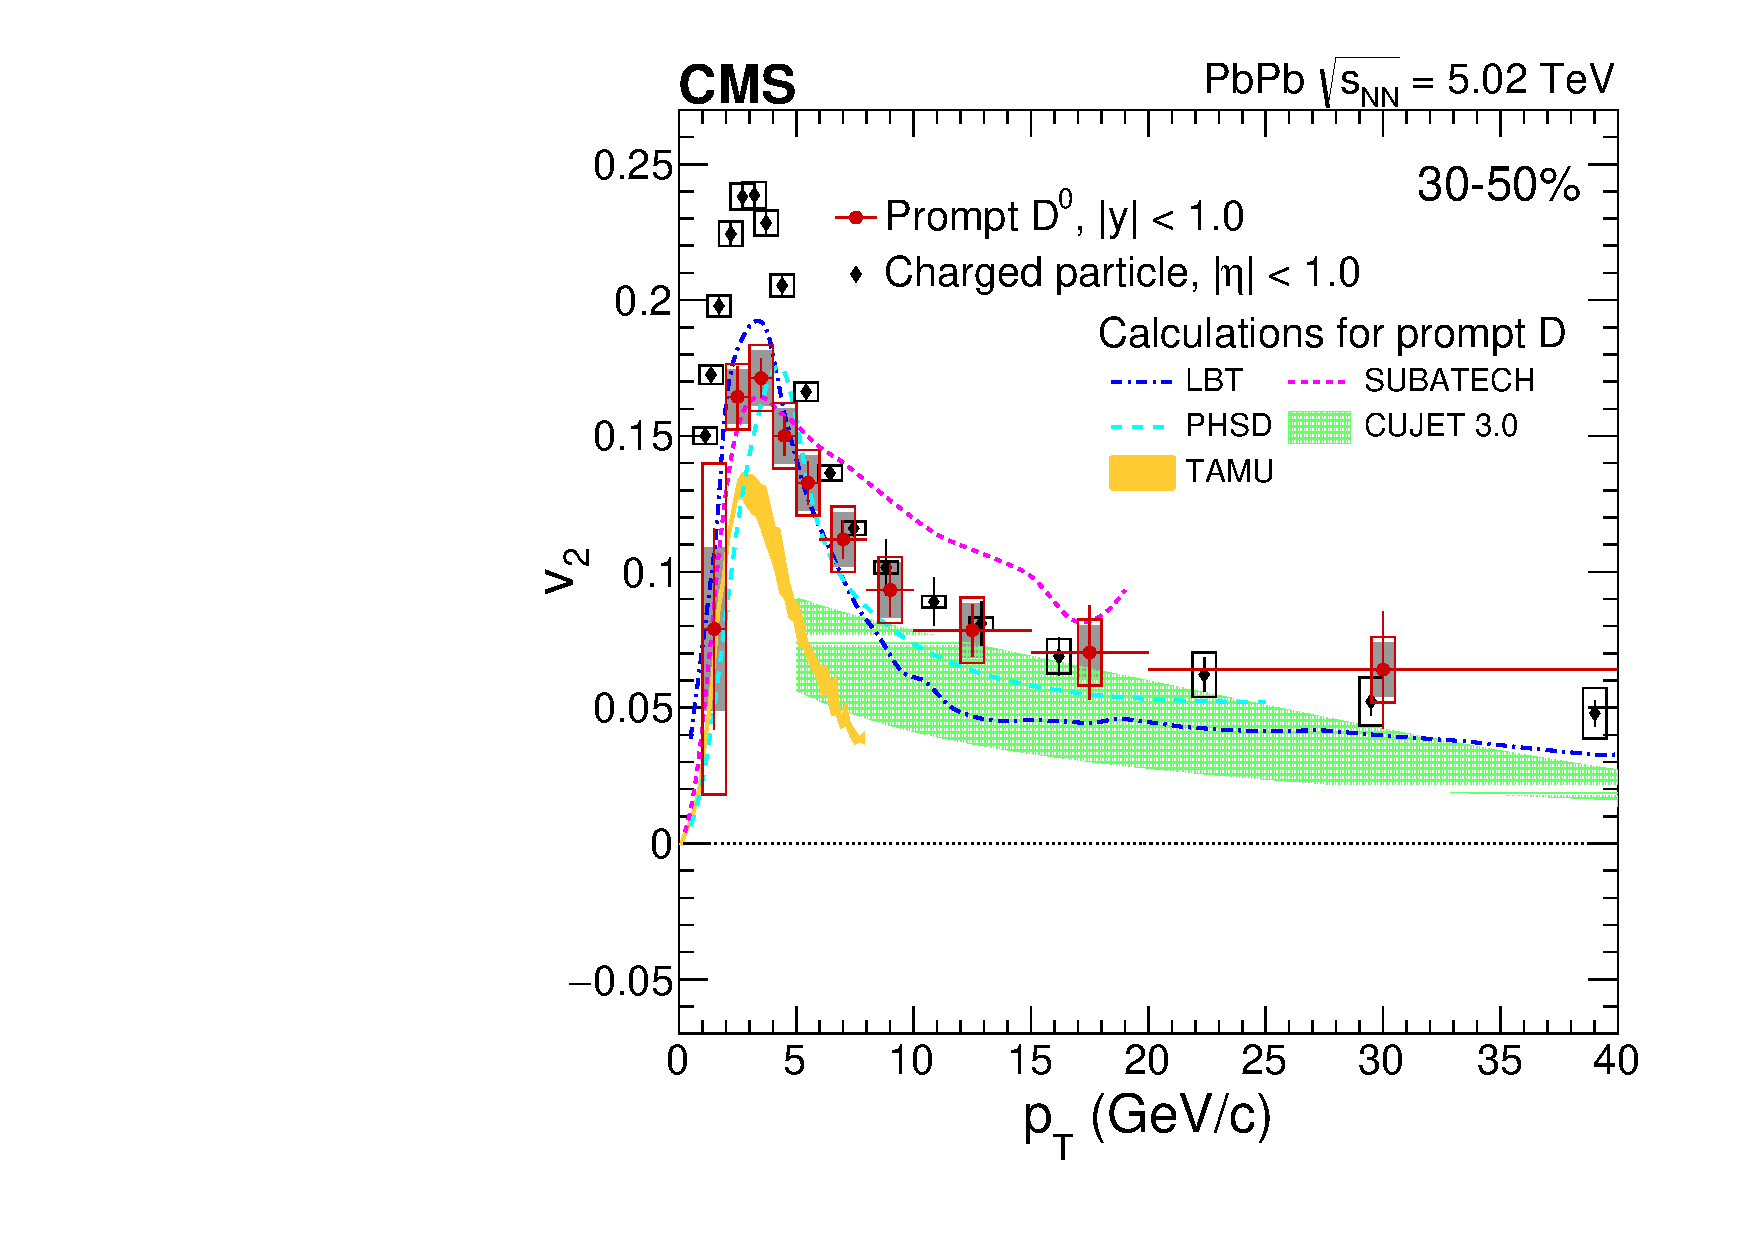
\includegraphics[width=.32\textwidth]{Plots/Dv2CMS3050.pdf}
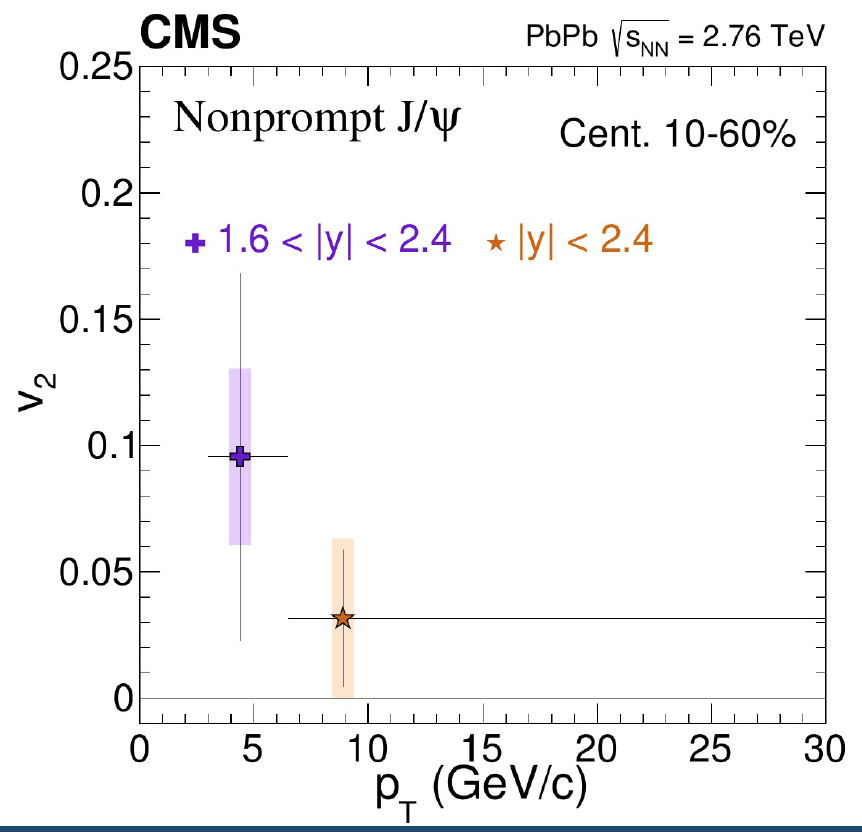
\includegraphics[width=.22\textwidth]{Plots/v2NonPromptPbPbCMS.png}
\caption{Please write your figure caption here}
\label{Dvn}     
\end{figure}


\section{A few words on the future}
\label{AAmeasurements}
In the last few years, impressive results were obtained in the sector of heavy-flavour observables in heavy-ion collisions, moving our field to an exciting era of high-precision measurements. 
Although a first quantitative understanding of heavy-flavour phenomena was achieved, a long way is still ahead in order to be able to use heavy-flavour observables to improve our understanding of the 
the properties of the Quark-Gluon Plasma. The plan for the next years of the experimental community in my opinion should be exploiting the new high-luminosity runs at RHIC and LHC and the 
upgraded detectors to improve the precision of the traditional observables but also provide new more differential observables (like D-hadron, D-jet, D-$\rm \bar{D}$ correlations, D-meson event-shape engineering measurements) 
that can contraints better the mechanisms of heavy-flavour production and the mechanisms of in-medium energy loss.  A better and quantitative understanding of the microscopic mechanisms of heavy-quark interaction with the 
medium (energy loss mechanisms and hadronisation mechanisms in particular) is a pre-requisitive in order to use theoretical calculations to derive fundamental properties of the medium like the transport coefficient or 
the diffusion coefficients. At the same time, measurements of heavy-flavour productions in smaller systems should be exploited to better understanding the properties and the nature of the collective phenomena that 
were observed in pp and proton-nucleus collisions. 

%%%%%%%%%%%%%%%%%%%%%%%%%
\begin{thebibliography}{}
\bibitem{saporegravis} A. Andronic et al., Eur. Phys. J. C 76 (2016) 107, doi:10.1140/epjc/s10052-015-3819-5, arXiv:1506.03981. 
\end{thebibliography}
\end{document}

\end{figure}


% end of file template.tex

%<div id='footer'><table width='100%'><tr><td class='right'><a href='http://fusioninventory.org/'><span class='copyright'>FusionInventory 9.1+1.0 | copyleft <img src='/glpi/plugins/fusioninventory/pics/copyleft.png'/>  2010-2016 by FusionInventory Team</span></a></td></tr></table></div>